%--------------------------------------------------------------------
% Эта преамбула с комментариями для написания лабораторных работ по
% физике. В еe основе информация из книги С. М. Львовского "Набор и
% верстка в пакете Latex", а также материалы по курсу "Документы и
% презентации в Latex" от ВШЭ https://www.coursera.org/learn/latex. Ну
% и мой опыт (1 год и 16 лабораторных работ + 2 Вопроса по выбору)
% Автор - Баринов Леонид
% Дата - 06.08.2019
%--------------------------------------------------------------------
%--------------------------------------------------------------------
% Для начала необходимо определиться с типом документа. Оптимальный
% (на мой взгляд) вариант - article. Также существуют типы book,
% report, proc и другие. Также в необязательном аргументе можно
% указать тип страницы и размер шрифта. Стандарт по умолчанию - А4 и
% 12 (иногда 10) шрифт. Необязательный аргумент шрифта может принимать
% только 3 параметра - 10, 11, 12 (pt).

\documentclass[a4paper, 12pt]{article}

%--------------------------------------------------------------------
% Чтобы использовать другие размеры шрифта используется пакет
% extsizes. Он позволяет указывать в \documentclass такие размеры - 8,
% 9, 10, 11, 12, 14, 17, 20 (pt). При указании других размеров могут
% возникать различные проблемы.

\usepackage{extsizes}

%--------------------------------------------------------------------
% Необходимо определиться с кодировкой документа. Идеального варианта
% для русского языка не существует - каждый чем-то немного плох. Для
% особо интересующихся - Приложение И в 5 издании книги Львовского. Я
% воспользовался вариантом, предлагаемым на курсе по Latex от ВШЭ.

\usepackage[T2A]{fontenc}
\usepackage[utf8]{inputenc}

%--------------------------------------------------------------------
% Для соблюдения типографских традиций (оказывается такие существуют)
% различных стран создан пакет babel. Самое заметное его действие -
% latex научиться переносить слова того языка, который вы укажите.
% Можно указать несколько языков через запятую. Основной язык
% документа указывается последним.

\usepackage[english,russian]{babel}

%--------------------------------------------------------------------
% Перейдем к заданию полей документа. Есть несколько способов, но
% самый простой из них - это воспользоваться пакетом geometry, который
% позволяет определить все поля документа (начиная с краев листа, что
% важно, так как некоторые другие способы позволяют это сделать только
% косвенно)

\usepackage{geometry}
\geometry{top=25mm}
\geometry{bottom=35mm}
\geometry{left=35mm}
\geometry{right=20mm}

%--------------------------------------------------------------------
% От полей логично перейти к колонтитулам. Тут нам поможет пакет
% fancyhdr. Для него существует 6 колонтитулов - верхний, левый;
% верхний, по центру; верхний, правый и такие же нижние. По умолчанию
% номер страницы находится снизу по центру, а также существует
% линейка, очерчивающие верхний колонтитул. Мне показалось интересным
% сделать колонтитулы схожие с колонтитулами в лабнике. 

\usepackage{fancyhdr}
\pagestyle{fancy}
\renewcommand{\sectionmark}[1]{\markboth{#1}{}} 
% \renewcommand{\headrulewidth}{0mm} % Если необходимо убрать линейку,
% или изменить ее длину
% \lfoot{} % Нижний левый
% \rfoot{} % Нижний правый
% \rhead{} % Верхний правый
% \chead{} % Верхний в центре
\lhead{\thepage} % Номер страницы в левом верхнем углу
\cfoot{} % Оставить нижний колонтитул без цифры

%--------------------------------------------------------------------
% Самое время научиться работать с формулами. А точнее добавить пакеты
% от Американского математического общества, которые позволять
% пользоваться большим количеством математических символов.

\usepackage{amsmath,amsfonts,amssymb,amsthm,mathtools}

%--------------------------------------------------------------------
% Также очень хочется пользоваться русскими буквами в формулах, для
% этого подключаем пакет mathtext, который добавляет окружение
% \text{}. Внутри него можно писать русские буквы в математическом
% режиме.

\usepackage{mathtext}

%--------------------------------------------------------------------
% Большим преимуществом вашего pdf документа будет возможность поиска
% в нем по словам или буквами. (Например, в Ивановнике это
% невозможно)

\usepackage{cmap}

%--------------------------------------------------------------------
% Куда же в физике без картинок и графиков? Давайте исправим
% эту недоработку

\usepackage{graphicx}
\graphicspath{images/} % Необходимо, если рисунки
% находятся в другой папке

%--------------------------------------------------------------------
% graphicx не позволяет вставлять обтекаемые рисунки, но на
% практике они очень нужны. Для этого существует пакет wrapfig

\usepackage{wrapfig}

%--------------------------------------------------------------------
% latex вставляет рисунки по определенному алгоритму. Его,
% конечно, можно менять, но это не настолько просто. Как
% правило, хочется, чтобы картинка располагалась там, где мы это
% указали в коде. Для этого существует несколько пакетов, один из
% них floatrow. Он позволяет для окружения figure указывать
% необязательный аргумент - H (именно большое h), что на latex'овском
% языке означает: вставить картинку здесь и только здесь. (даже если
% облик документа несколько пострадает)

\usepackage{floatrow}

%--------------------------------------------------------------------
% По правилам оформления рисунок всегда должен быть подписан. Для
% этого существует команда \caption{}. Но обычные настройки caption
% меня не совсем устроили. Хотелось сделать подпись меньше
% основного шрифта, а также слово Рис жирным и использовать
% разделитель точку, а не двоеточие. В этом помогает пакет,
% который называется caption (совпадение?)

\usepackage[margin=10pt,font=small,labelfont=bf,labelsep=period]{caption}

%--------------------------------------------------------------------
% Последним важным пунктом остались таблицы. Ведь куда-то нужно
% заносить результаты измерений. На данный момент во время выполнения
% лабораторных работ я заношу результаты в таблицу excel, а потом с
% помощью сайта www.tablesgenerator.com превращаю в таблицу latex и
% дооформляю.

\usepackage{array,tabularx,tabulary,booktabs}

%--------------------------------------------------------------------
% После excel есть ощущения, что везде объединить колонки или строки
% легко. В latex не совсем так. Помогают пакеты multirow, multicol. 

\usepackage{multirow}
\usepackage{multicol}

%--------------------------------------------------------------------
% Иногда могут потребоваться длинные таблицы на несколько страниц.
% Обычные таблицы latex воспринимает как одну букву. И
% становиться понятно, почему возникают проблемы при переносе
% обычной таблицы. (Ведь нельзя же перенести одну букву!). Поэтому
% вместо обычной таблицы нужна длинная таблица.

\usepackage{longtable}

%--------------------------------------------------------------------
% Часто в таблице хочется сделать перенос текста или формулы. Просто
% так это сделать не получиться из-за синтаксиса tabular. Для этого
% каждый раз необходимо создавать новое окружение tabular, что
% утомительно. Поэтому можно ввести команду \specialcell
% (назвать можно по-любому)
    
\newcommand{\specialcell}[2][c]{%
	\begin{tabular}[#1]{@{}c{}}#2\end{tabular}}

%--------------------------------------------------------------------
% Когда в таблице много колонок и строк, кажется, что они находятся
% слишком близко к друг другу. Можно переопределить
% несколько параметров, чтобы выглядело лучше. Это можно сделать либо
% в преамбуле, либо непосредственно в документе. Первое
% переопределение отвечает за интервал между строками, второе за
% интервал между колонками

% \renewcommand{\arraystretch}{1.8} 
% \renewcommand{\tabcolsep}{1cm} 

%--------------------------------------------------------------------
% В русской типографской традиции принято начинать каждый новый абзац
% с красной строки. Даже первый после заголовка (или подзаголовка).
% Чтобы каждый раз не ставить красную строку вручную существует пакет
% indentfirst

\usepackage{indentfirst}

%--------------------------------------------------------------------
% Некоторые модификаторы начертания

\usepackage{soul}
\usepackage{soulutf8}
 
\usepackage{mathrsfs}
\begin{document}
\thispagestyle{empty}
\begin{center}
    \textit{Федеральное государственное автономное образовательное\\ учреждение высшего образования }

    \vspace{0.5ex}

        \textbf{«Московский физико-технический институт\\ (национальный исследовательский университет)»}
\end{center}

\vspace{10ex}

\begin{center}
    \vspace{13ex}

    \so{\textbf{Лабораторная работа №_._._}}

    \vspace{1ex}

    по курсу общей физики

    на тему:

    \textbf{\textit{<<>>}}

    \vspace{30ex}

    \begin{flushright}
        \noindent
        \textit{Работу выполнил:}\\  
        \textit{Баринов Леонид \\(группа Б02-827)}
    \end{flushright}
    \vfill
    Долгопрудный \\2019
\newpage
\setcounter{page}{1}
\fancyhead[R]{\nouppercase{\leftmark}}	
\end{center}

\section{Аннотация}
В работе будет изучена вольт-амперная
характеристика тлеющего заряда, а также
изучены свойства плазмы методом зондовых
характеристик.
\section{Теоретические сведения}
При нагревании газа молекулы распадаются
на атомы, а затем атомы распадаются на
электроны и ионы, так что газ становится
ионизованным, представляя собой смесь из
свободных электронов и ионов, а также
нейтральных частиц.

Степень ионизации -- отношение
числа ионизованных атомов к их полному
числу. При высокой степени ионизации газ
начинает обладать высокой
электропроводностью и, в отличие от
нейтральных газов, взаимодействует с
электрическими и магнитными полями.
Кроме того, заряженные частицы в таком
газе стремятся распределиться в
пространстве таким образом, чтобы
установилась локальная
квазинейтральность, то есть равенство
концентрация положительных и
отрицательных частиц, нарушаемое
тепловыми флуктуациями только в
микроскопических масштабах. Такое
состояние ионизованного газа называется
плазмой.

Основные параметры, характеризующие
плазму: плотности составляющих ее частиц
-- электронов -- $n_e$, ионов -- $n_i$ и
нейтральных частиц -- $n_0$, их
температуры~-- соответственно $T_e, T_i,
T_0$. 

Оценим размер области, внутри которой
могут существовать заметные
электрические поля. Рассмотрим
пространство вокруг иона, имеющего
положительные заряд и поэтому
притягивающего электроны, поле которых
противоположно по знаку полю иона. Ион
<<экранируется>> электронами, поля
убывает сильнее чем $1/r^2$. Тепловое
движение мешает полной <<экранировки>>
иона.

Запишем выражение для $\text{div}\, E$,
используя потенциал $\varphi$ и оператор
Лапласа $\Delta$ в сферической системе
координат.
\begin{equation}
    \frac{d^2\varphi}{dr^2}+\frac{2}{r}\frac{d\varphi}{dr}
    = -4\pi\rho
\end{equation}


Распределение электронов, а значит и их
пространственного заряда, подчиняется
формуле Больцмана:
\begin{equation}
    \rho_e=-ne\cdot e^{e\varphi/kT_e}
\end{equation}

Будем считать ионы бесконечно тяжелыми,
то есть неподвижными ($M \gg m_e$), что
как показывают точные расчеты, не меняет
ответа по порядку величины. То есть
$\rho_i = const$ и равно своему значению
в области $\varphi = 0$, где он равен и
противоположен по знаку
пространственному заряду электронов
\begin{equation}
    \rho_i = ne
\end{equation}
Подставим (2) и (3) в (1):
\begin{equation}
    \frac{d^2\varphi}{dr^2}+\frac{2}{r}\frac{d\varphi}{dr}
    = -4\pi n e \left[ 1- e^{e\varphi/k
    T_e} \right] 
\end{equation}
Рассмотрим случай, когда 
\[
\frac{e\varphi}{kT_e} \ll 1
\]
Разложим экспоненту в ряд, и получаем
линейное уравнение 
\begin{equation}
    \frac{d^2\varphi}{dr^2}+\frac{2}{r}\frac{d\varphi}{dr}
    = \frac{1}{r_D^2} \varphi,  
\end{equation}
где введено обозначение
\begin{equation}
    r_D = \sqrt{\frac{kT_e}{4\pi n e^2}}
\end{equation}
Решение уравнение (5) примет вид:
\begin{equation}
    \varphi = \frac{Ze}{r}e^{-r/r_D}
\end{equation}
$r_D$ -- дебаевский радиус экранирования
(радиус Дебая, дебаевская длина)

Введем более строгое определение плазмы.
Плазмой называется ионизованный газ,
дебаевский радиус которого $r_D$
существенно меньше характерного размера
$l$ объема, занимаемого этим газом, то
есть
\[
    \sqrt{\frac{k T_e}{4\pi n e^2}} \ll
    l.
\]

Это означает, что энергия взаимодействия
двух незаряженных частиц в плазме
существенно меньше их тепловой энергии,
то есть что плазма является газом,
причем идеальным.

Число частиц $N_D$ в дебаевской сфере
можно оценить с помощью формулы (6),
подставляя в нее вместо истинного
среднее число частиц 
\begin{equation}
    N_D \approx n\frac{4}{3}\pi r_D^3
    \approx
    \frac{(kT_e)^{3/2}}{n^{1/2}e^3}
\end{equation}
    
\begin{wrapfigure}{r}{0.28\linewidth}
    \vspace{-3ex}
    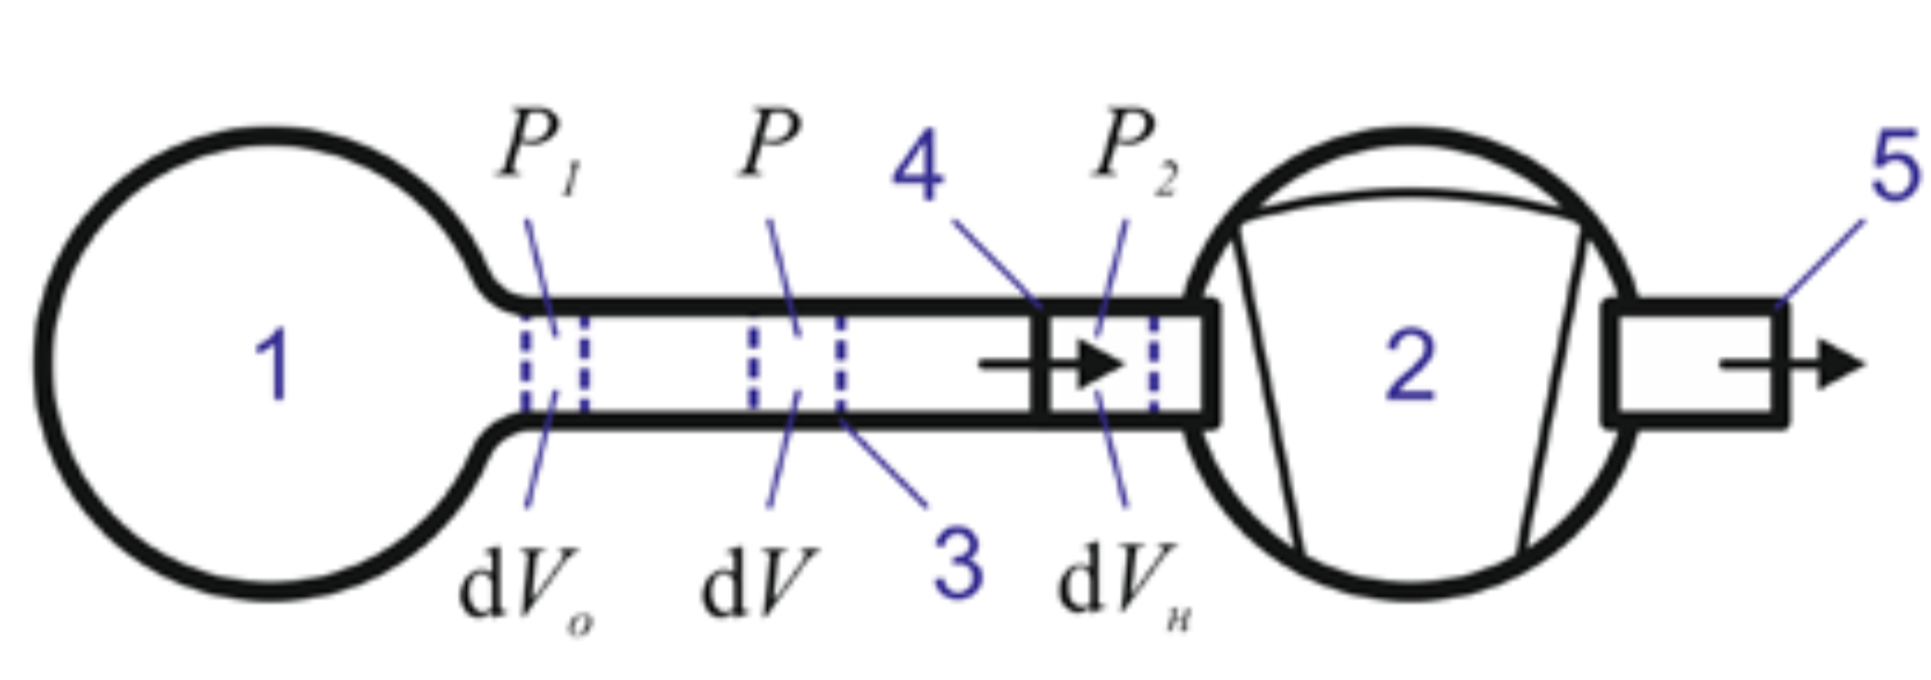
\includegraphics[width=\linewidth]{1}
    \captionsetup{justification=centering}
    \caption{}
\end{wrapfigure}

Другой важнейшей характеристикой плазмы
является плазменная или ленгмюровская
частота, выражение для которой и её
смысл можно получить из следующих
соображений. Выделим в плазме объём в
виде параллелепипеда, изображённого на
рис. 1. Сместим все электроны на
расстояние $x$ относительно ионов (ионы
занимают объём, изображённый сплошными,
а электроны — пунктирными линиями).
Пусть плотность электронов (и ионов)
равна $n$; ионы для простоты будем считать
однозарядными. Легко видеть, что в
результате такого смещения на гранях
параллелепипеда возникнут поверхностные
заряды:
\begin{equation}
    \sigma = n e x
\end{equation}
Вследствие этого появится электрическое
поле:
\begin{equation}
    E=4 \pi \sigma = 4\pi n e x
\end{equation}
Это поле действует на электроны,
придавая им ускорение, равное 
\begin{equation}
    \frac{d^2x}{dt^2} = \frac{eE}{m} = - 
    \frac{4\pi n e^2}{m}x
\end{equation}
Уравнение (11) определяет плазменную
(ленгмюровскую) частоту, коллективных
колебаний электронов:
\begin{equation}
    \omega_p = \sqrt{\frac{4\pi n
    e^2}{m}} = 5,65\cdot 10^4
    \sqrt{n(\text{см}^{-3})}
\end{equation}

Плазменная частота задает естественный
масштаб времени для плазмы: это — время
отклика на флуктуацию плотности заряда в
плазме. Учитывая это, дебаевский радиус
экранирования можно интерпретировать
следующим образом. Пусть какая-то группа
электронов получила направленную
скорость, равную тепловой: $\upsilon =
\sqrt{k T_e/m_e}$.
При этом, как легко можно убедиться,
обращаясь к формулам (12), (6), за
время, равное $\omega_p^{-1}$, эта группа
электронов пройдёт в направлении
полученной скорости до полной остановки
расстояние, как раз равное дебаевской
длине, то есть
\begin{equation}
    r_D = \frac{\upsilon}{\omega_p}    
\end{equation}

Таким образом, дебаевская длина — это
амплитуда ленгмюровских колебаний
плазмы, возбуждаемых тепловыми
флуктуациями. Эта амплитуда и является
масштабом нарушения квазинейтральности
плазмы в отсутствие внешнего поля.

Как следует из (12), плазменная
частота определяется только плотностью
электронов (и универсальными
постоянными). Можно строго доказать, что
она не зависит от величины и формы
рассматриваемого объёма и является,
таким образом, локальной характеристикой
плазмы. Плазменная частота является не
единственной — но важнейшей —
характерной частотой плазмы. Она
определяет коллективное движение
электронов относительно ионов.

В заключение этого пункта сделаем
следующее замечание. Формула для
дебаевского радиуса (6) не учитывает
движение ионов. Если считать, что ионы
тоже распределяются в поле пробного
заряда по Больцману с температурой $T_i$,
то в приближении $e\varphi \leqslant k
T_i$, вместо
формулы (6) получим
\begin{equation}
    r_D = \sqrt{\frac{k}{4\pi n
    e^2}\frac{T_e T_i}{T_e + T_i}},
\end{equation}
то есть вместо $T_e$
в формулу для дебаевского радиуса войдёт
приведённая температура. В частности,
при $T_e = T_i$ в знаменателе под корнем
появляется двойка, а при $T_e \gg T_i$, что
имеет место для плазмы газового разряда
(тлеющего), в формуле (6) вместо $T_e$ 
будет стоять $T_i$.

\subsubsection*{ВАХ газового промежутка}

Экспериментально ВАХ газового проводника
— например, промежутка между двумя
электродами, помещёнными в стеклянную
трубку, заполненную газом, — снимают с
помощью схемы, представленной на рис.
2. Цепь содержит источник постоянного
напряжения $\mathscr{E}$ величину
которого можно изменять в пределах
примерно от 100 В до нескольких кВ, и
переменное сопротивление $R$, называемое
балластным, или нагрузочным.

\begin{wrapfigure}{l}{0.4\linewidth}
    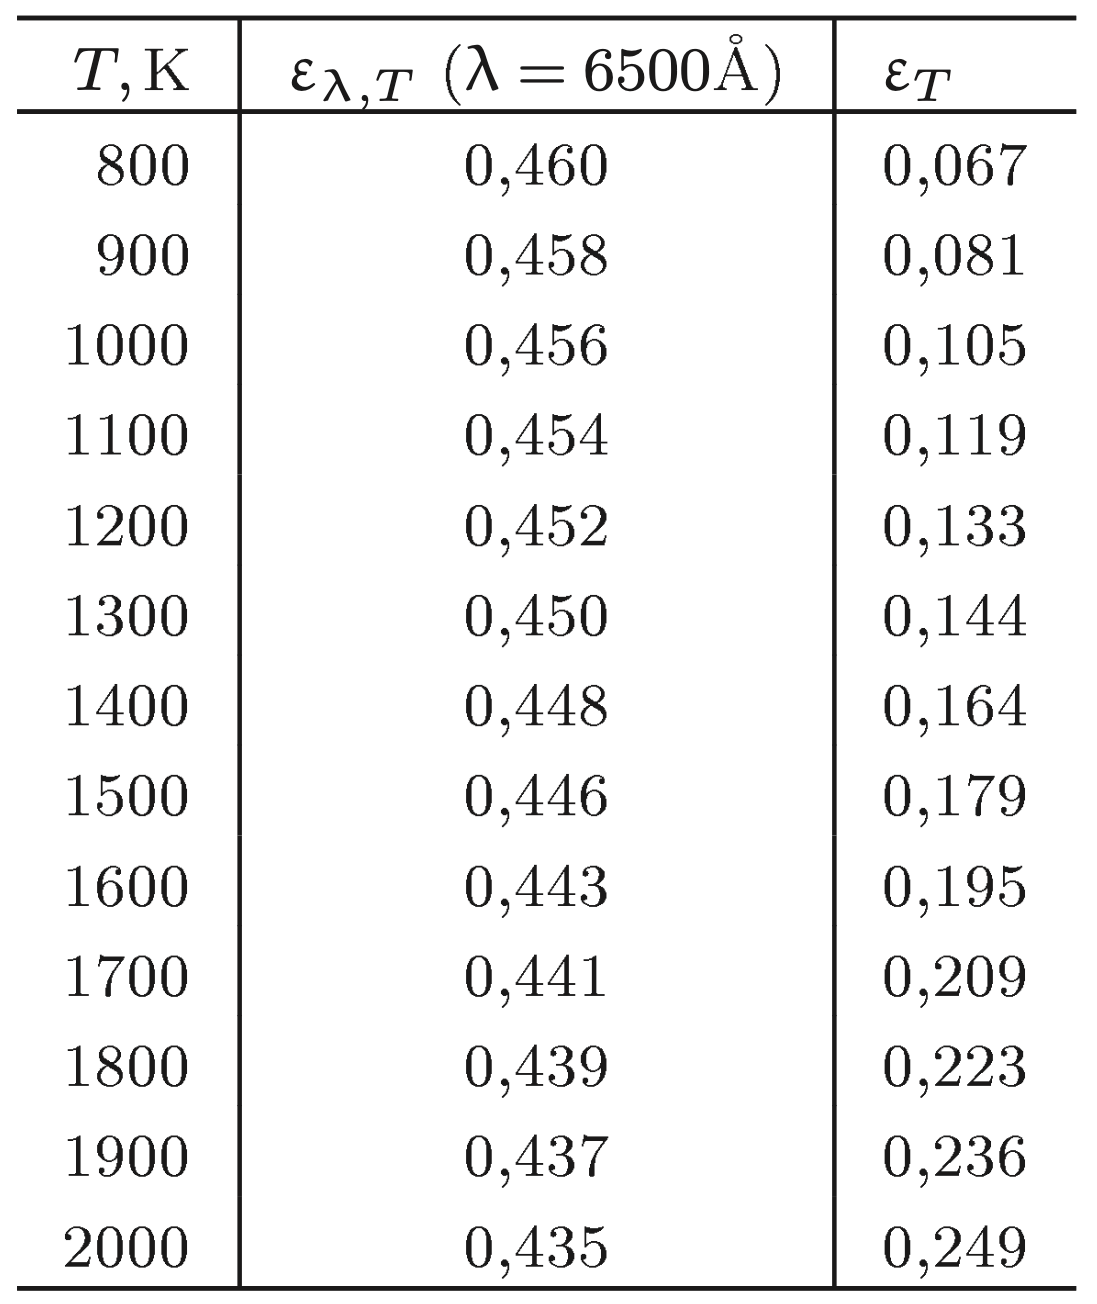
\includegraphics[width=\linewidth]{2}
    \captionsetup{justification=centering}
    \caption{Схема для снятия ВАХ
    газового промежутка}
\end{wrapfigure}
Это
сопротивление необходимо для ограничения
тока в цепи и стабилизации разряда на
участках с отрицательным
дифференциальным сопротивлением. Дело в
том, что на этих участках разряд
неустойчив и ток имеет тенденцию
неограниченно нарастать. Можно показать,
что для устойчивости разряда сумма
отрицательного и положительного
сопротивлений такой цепи должна быть
положительной, то есть в точке
пересечения с ВАХ нагрузочная прямая
должна иметь больший наклон, чем участок
кривой ВАХ (рис. 5.7).

Вид ВАХ для конкретного газового
проводника зависит от ряда условий,
прежде всего от давления газа. На рис.
3 представлена полученная
экспериментально с помощью схемы рис.
2 ВАХ разряда в неоне при давлении 1,3
мбар между плоскими медными электродами
площади 10 см$^2$, расположенными на
расстоянии 50 см, а также типичная
нагрузочная прямая. Поскольку здесь нет
специального внешнего ионизатора
(внешняя ионизация создаётся только
естественным радиоактивным излучением и
космическими лучами), начальный участок
характеристики несамостоятельного
разряда (участок ОА на рис. 5.3)
соответствует столь малым токам, что на
графике его не удаётся изобразить.
Характеристика начинается сразу с
участка АБ, соответствующего току
насыщения (участок АБ на рис. 5.3) и
режиму газового усиления. В точке В
происходит пробой и начинается
самостоятельный разряд, который на всём
горизонтальном участке характеристики ВГ
соответствует тёмному таунсендовскому
разряду. 

\begin{figure}[H]
    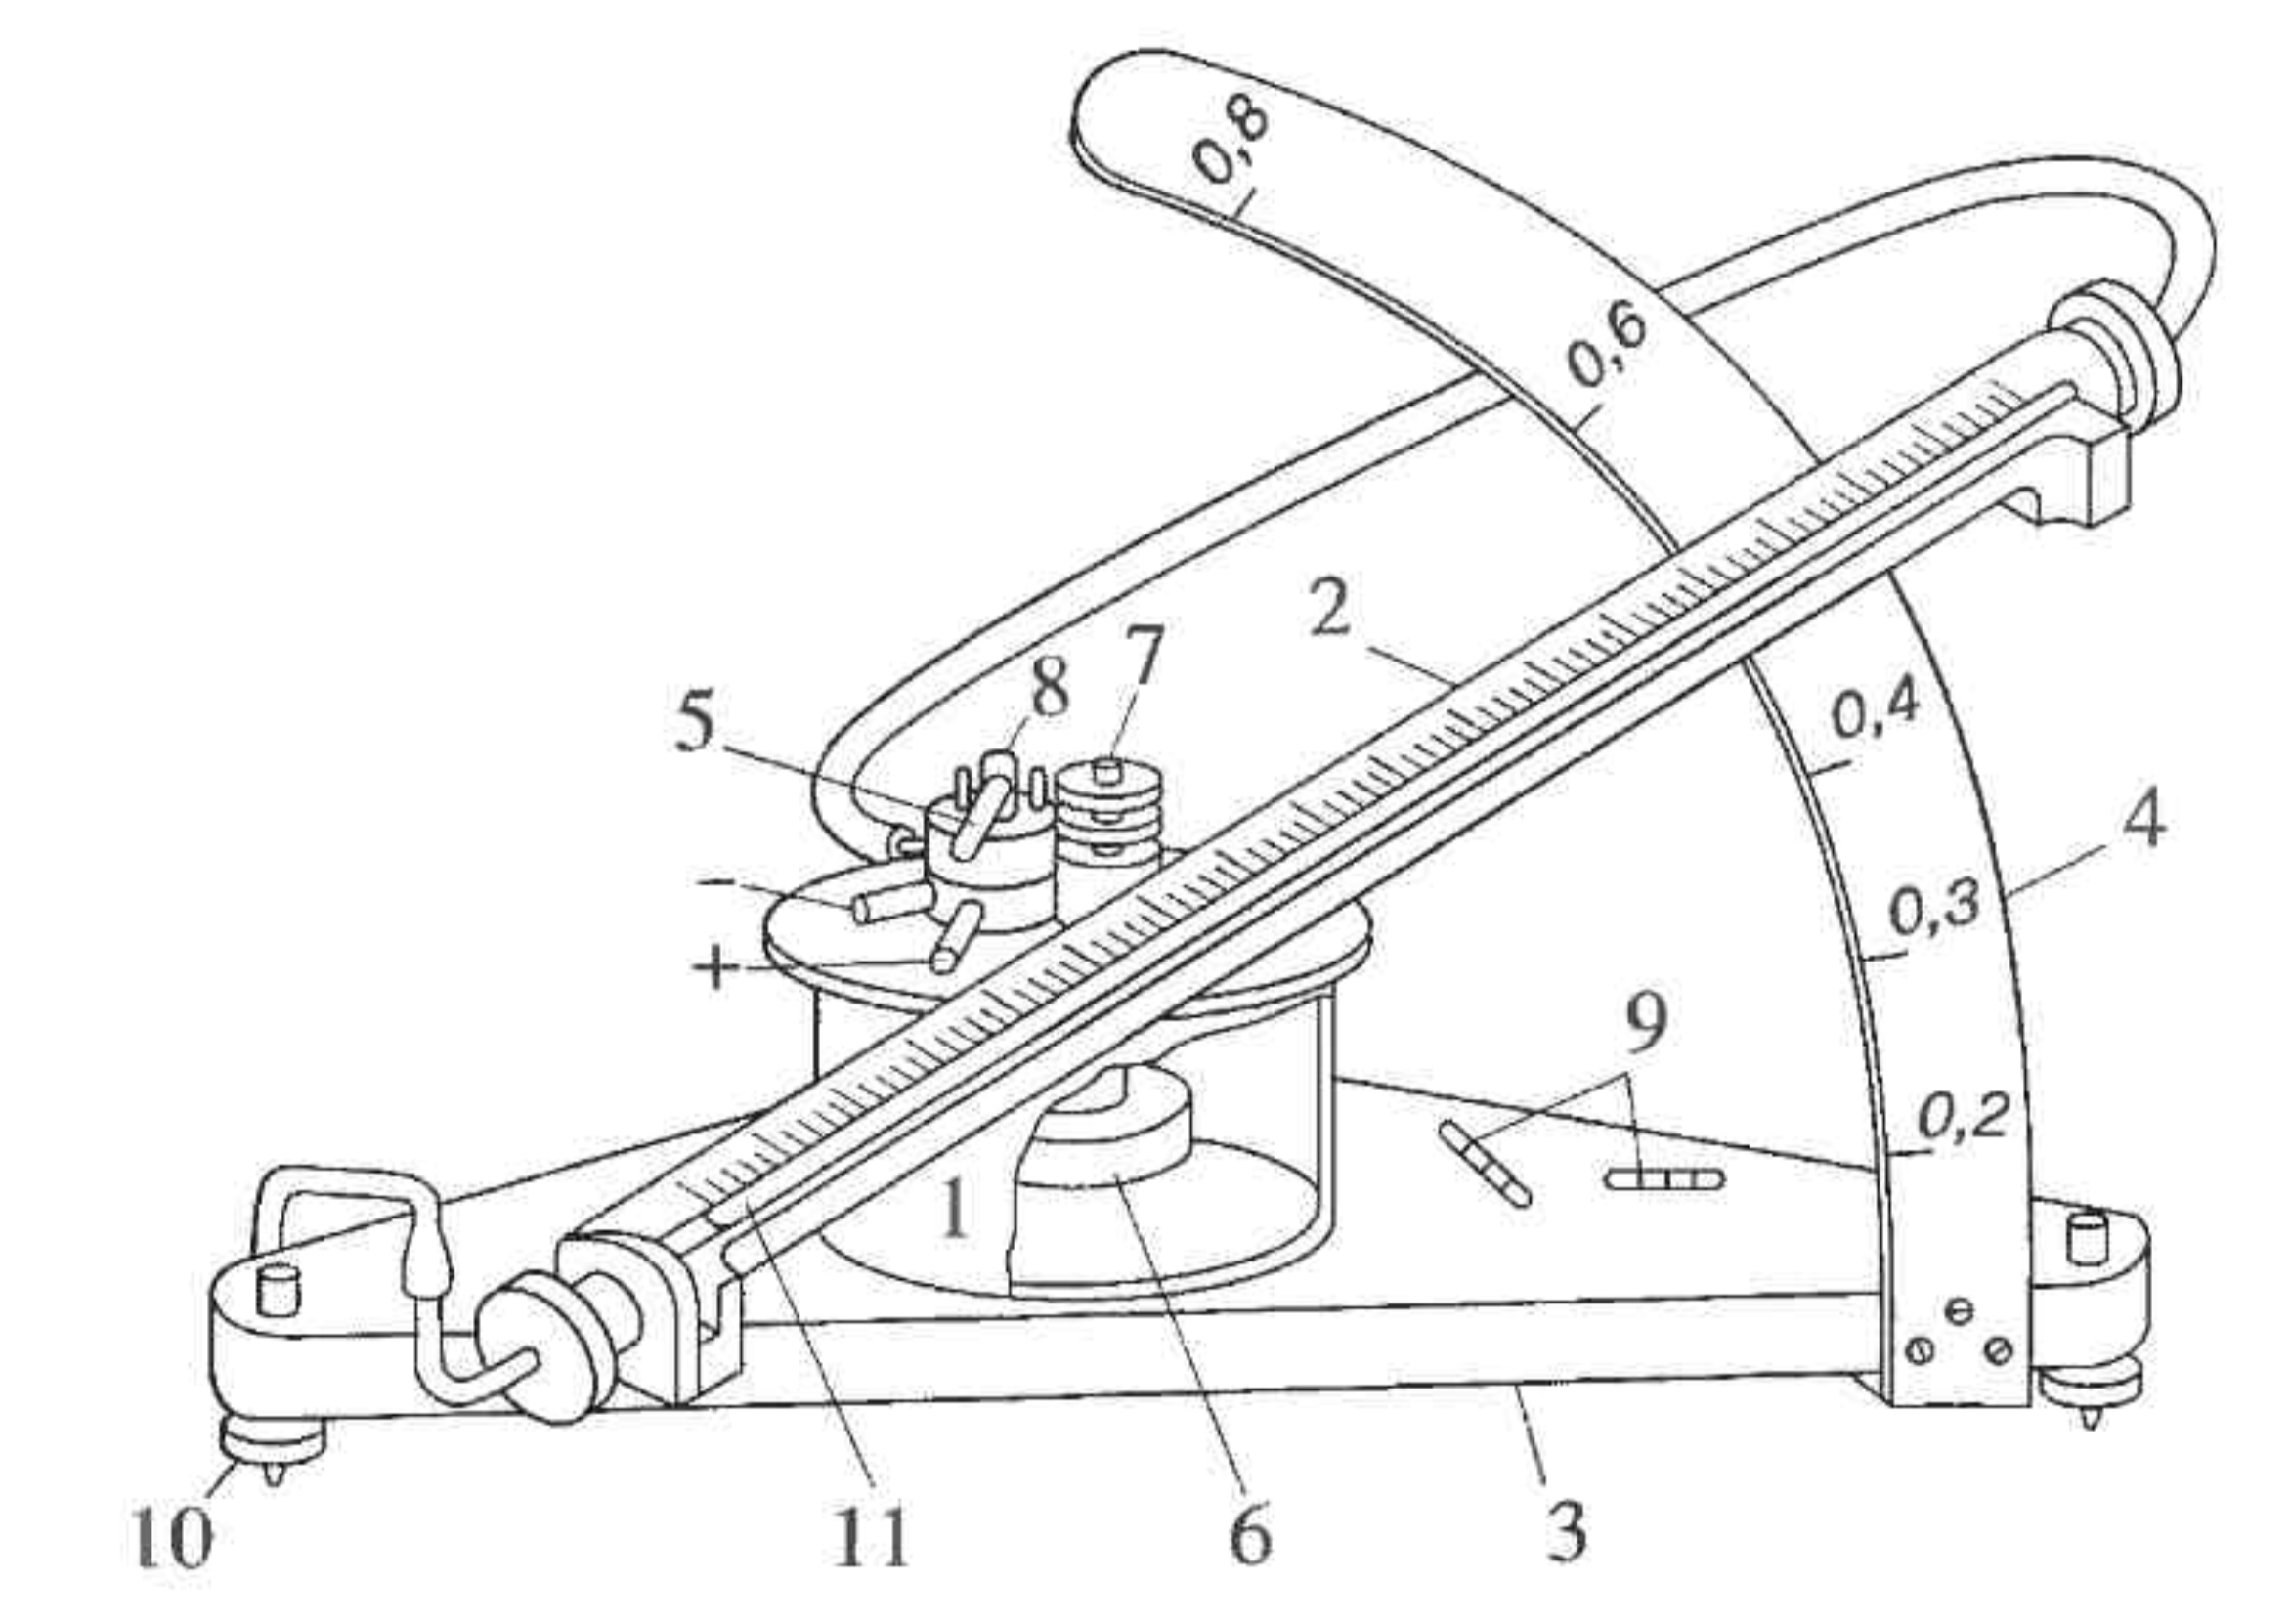
\includegraphics[width=0.9\linewidth]{3}
    \captionsetup{justification=centering}
    \caption{ВАХ разряда в неоне при
    давлении $1,3 \ \text{мбар}$ и
нагрузочная прямая}
\end{figure}

Участок характеристики ГДЕЖ
соответствует тлеющему разряду, 
причём его падающая часть ГД называется
поднормальным тлеющим разрядом,
горизонтальная часть ДЕ — нормальным
тлеющим разрядом и остальная часть ЕЖ —
аномальным тлеющим разрядом. Далее идёт
падающий участок ЖЗ, который можно
получить при маленьких сопротивлениях и
сильноточных источниках напряжения. Он
соответствует переходу к дуговому
разряду. Заметим, что при больших
давлениях газа (атмосферном и больше)
после пробоя сразу устанавливается
дуговой разряд.


\begin{wrapfigure}[29]{r}{0.4\linewidth}
    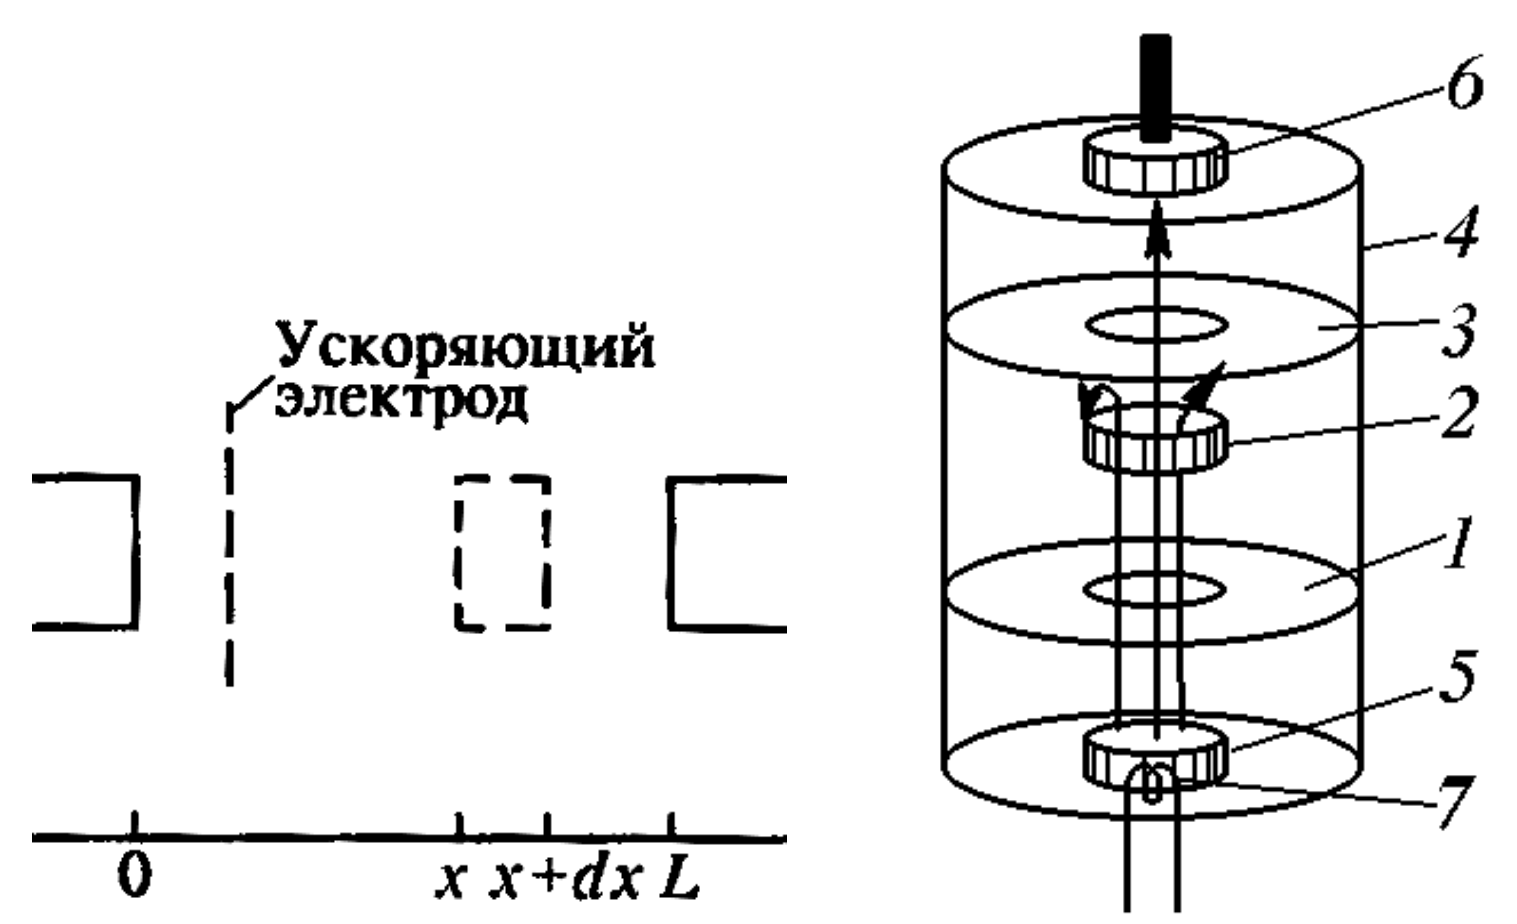
\includegraphics[width=\linewidth]{4}
    \captionsetup{justification=centering}
    \caption{Структура тлеющего разряда
    и распределение по длине основных
характеризующих его величин}
\end{wrapfigure}

На рис. 4 представлена качественная
картина тлеющего разряда в длинной
стеклянной трубке, а также приведены
зависимости основных величин,
характеризующих разряд, от продольной
координаты. Это интенсивность свечения,
потенциал и напряжённость электрического
поля, электронный и ионный токи,
электронная и ионная плотности и полная
плотность объёмного заряда.
Видно, что разряд состоит из ряда
чередующихся светлых и тёмных поперечных
полос. Поскольку все процессы в разряде
связаны со столкновениями электронов с
атомами газа, расстояния от катода до
этих полос определяются числом
укладывающихся на них длин пробега
электронов. Поэтому характерные размеры
полос увеличиваются с уменьшением
давления. Непосредственно к катоду
прилегает узкое астоново пространство,
затем идёт слой катодного свечения, а
затем — тёмное катодное пространство.
Далее следует область отрицательного
свечения, переходящая в тёмное фарадеево
пространство. За ним начинается
светящийся положительный столб,
заканчивающийся у анода тёмным анодным
пространством, переходящим на аноде в
узкий слой анодного свечения.

Как правило, самой яркой бывает область отрицательного свечения, имеющего для воздуха голубоватый цвет, за что разряд и получил своё 
название -- тлеющий.

Рассмотрим явления, происходящие при
внесении в плазму уединенного проводника
-- зонда. Пусть электрический потенциал
зонда вначале равен потенциалу той точки
плазмы, в которую будет помещен зонд.
Поступающие на зонд токи электронов и
ионов в этом случае равны
\begin{align}
    I_{e0} = \frac{n \langle \upsilon_e
    \rangle}{4}e S \\
    I_{i0} = \frac{n \langle \upsilon_i
    \rangle}{4}e S
\end{align}
где $\langle \upsilon_e \rangle$ и
$\langle \upsilon_i \rangle$ -- средние
скорости электронов и ионов (которые в
силу квазинейтральности плазмы равны или
почти равны друг другу). Множитель $1/4
n \langle \upsilon \rangle$, согласно
кинетической теории, определяет число
ударов в секунду о единицу поверхности.

Оценим величину электронного и ионного
тока насыщения. Электронный ток
насыщения определяется формулой (15) и
формулой из МКТ
\begin{equation}
    \langle \upsilon_e \rangle =
    \sqrt{\frac{8kT_e}{\pi m_e}}
\end{equation}
В итоге получаем
\begin{equation}
    I_{e\text{н}} = \frac{1}{4} n e S
    \langle \upsilon_e \rangle \approx
    \frac{1}{4} n e S \sqrt{\frac{8 k
    T_e}{\pi m_e}}
\end{equation}

Ионный ток насыщения по аналогичной
формуле оценивать не следует, поскольку
скорости ионов в окрестности зонда
определяются не температурой плазмы, а
разностью потенциалов между плазмой и
зондом:
\begin{equation}
    \upsilon_i \approx \sqrt{\frac{2 e
    U}{m_i}}
\end{equation}

Опыт показывает, что вместо формулы
(5.29) для вычисления этого тока лучше
применять полуэмпирическую формулу,
предложенную Бомом:
\begin{equation}
    I_{i\text{н}} = 0,4 n e S
    \sqrt{\frac{2 k T_e}{m_i}}
\end{equation}

\subsection*{Двойной зонд}
Двойным зондом называется система,
состоящая из двух одинаковых зондов,
расположенных на небольшом расстоянии
друг от друга. Между зондами создаётся
разность потенциалов, которая по
величине много меньше плавающего
потенциала $U_f$. При этом оба зонда имеют
относительно плазмы близкий к плавающему
отрицательный потенциал, т. е. находятся
на ионной ветви вольт-амперной
характеристики.

При отсутствии разности потенциалов ток
между зондами равен нулю. Рассчитаем
величину тока, проходящего через двойной
зонд вблизи точки $I = 0$. При небольших
разностях потенциалов ионные токи на оба
зонда равны ионному току насыщения и
компенсируют друг друга. Величина
результирующего тока целиком связана с
различием в электронных токах. Пусть
потенциал на первом зонде равен
\begin{equation}
    U_1 = -U_f + \Delta U_1
\end{equation}
а на втором
\begin{equation}
   U_2 = -U_f + \Delta U_2
\end{equation}

По предположения $\Delta U_1$ и $\Delta
U_2$ меньше $U_f$. Напряжение $U$ между
зондами равно
\begin{equation}
    U=U_2-U_1 = \Delta U_2 - \Delta U_1
\end{equation}
Найдем ток, приходящий на первый
электрод:
\begin{multline*}
    I_1 = I_{i\text{н}} + I_{e1} =
    I_{i\text{н}} - \frac{1}{4}n e S
    \langle \upsilon_e \rangle \cdot
    \exp \left[ \frac{e(-U_f + \Delta
    U_1)}{k T_e}  \right] = \\ =
    I_{i\text{н}} - \left\{ \frac{1}{4} n
    e S \langle \upsilon_e \rangle \exp
    \left(-\frac{e U_f}{k T_e}
        \right)\right\} \exp \left(\frac{e
    \Delta U_1}{k T_e}  \right)
\end{multline*}
Заметим теперь, что при $\Delta U_1 = 0$ 
(при $U_1 = U_f$) электронный и ионный
ток компенсируют друг друга. Это
означает, что заключенный в фигурные
скобки множитель равен $I_{i\text{н}}$.
Имеем поэтому
\begin{equation}
    I_1 = I_{i \text{н}} \left[ 1 - \exp
        \left( \frac{e \Delta U_1}{k T_e}  \right)\right]
\end{equation}
Аналогично
\begin{equation}
    I_2 = I_{i \text{н}} \left[ 1 - \exp
        \left( \frac{e \Delta U_2}{k T_e}  \right)\right]
\end{equation}

Заметим также, что зонды 1 и 2 соединены
последовательно и через них проходит
один и тот же ток $I$, но в разном
направлении. Положим
\begin{equation}
I_1 = - I_2 = I
\end{equation}

Выразим $\Delta U_1$ и $\Delta U_2$ из
(24) и (25) и заменим входящие в эти
выражения $I_1$ и $I_2$ через $I$ с
помощью (26):
\begin{align}
    \Delta U_1 = \frac{k T_e}{e} \ln
    \left(1 - \frac{I}{I_{i\text{н}}}
    \right) \\
    \Delta U_2 = \frac{k T_e}{e} \ln
    \left(1 + \frac{I}{I_{i\text{н}}}  \right)
\end{align}
Вычитая второе равенство из первого,
найдем
\begin{equation}
    U = \Delta U_1 - \Delta U_2 =
    \frac{k T_e}{e} \ln
    \frac{1-I/I_{i\text{н}}}{1+I/I_{i\text{н}}}
\end{equation}
Разрешая это равенство относительно $I$,
найдем
\begin{equation}
    I = I_{i\text{н}} \th \frac{e U}{2 k
    T_e}
\end{equation}

Эта формула может служить для
определения температуры электронов по
форме вольт-амперной характеристики
двойного зонда.

\begin{wrapfigure}{r}{0.4\linewidth}
    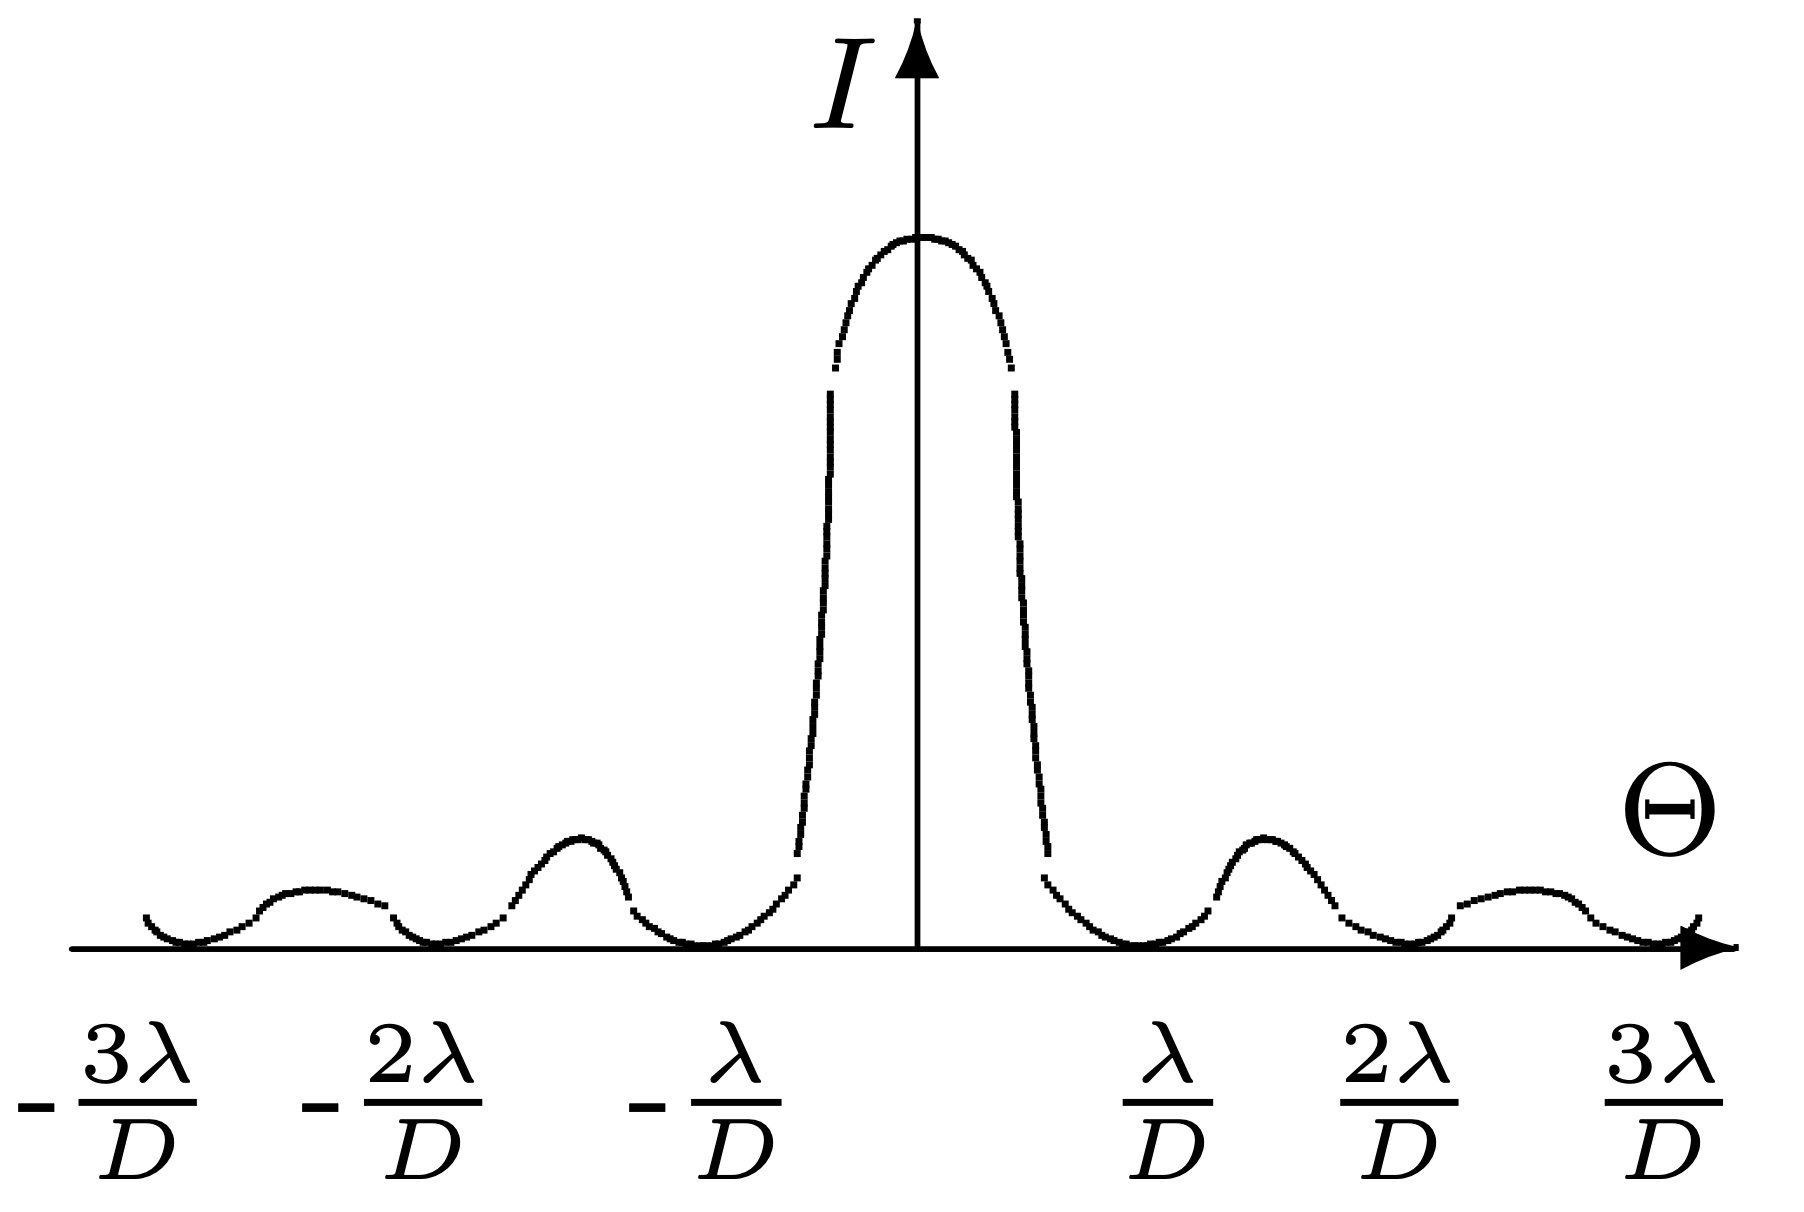
\includegraphics[width=\linewidth]{5}
    \captionsetup{justification=centering}
    \caption{Вольт-амперная
    характеристика двойного зонда}
\end{wrapfigure}

Наблюдаемая на опыте зависимость тока от
напряжения изображена на рис. 4. Эта
кривая отличается от (30) наклоном
асимптот в области больших $|U|$. 
Наклон асимптот в первом приближении
является линейным. Поэтому вместо (30)
лучше писать
\begin{equation}
    I = I_{i\text{н}} \th \frac{e U}{2 k
    T_e} + A U,
\end{equation}
где $A$ -- некоторая константа, величина
которой может быть найдена из опыта.



При обработке графика на рис. 5 сначала
находится $I_{i\text{н}}$ из пересечении
асимптот с осью $U = 0$. Затем, по наклону
асимптот, находится величина $A$. После
этого из (31) нетрудно определить $T_e$.
Дифференцируя эту формулу по $U$ в точке 
$U = 0$ и принимая во внимание, что при
малых аргументах $\th \alpha \approx
\alpha$, а при малых
наклонах кривой насыщения $A \rightarrow
0$, найдём

\begin{equation}
    k T_e = \frac{1}{2} \frac{e
    I_{i\text{н}}}{\frac{dI}{dU}\left|_{U=0}
\right.}
\end{equation}

\section{Оборудование}
\textbf{В работе используется:}
стеклянная гзоразрядная трубка,
наполненная изотопом неона,
высоковольтный источник питания (ВИП),
источник питания постоянного тока,
делитель напряжения, резистор,
потенциометр, амперметры, вольтметры,
переключатели.  

\subsubsection*{Экспериментальная установка}
Схема
установки для исследования плазмы
газового разряда в неоне представлена на
рис. 6. Стеклянная газоразрядная трубка
имеет холодный (ненакаливаемый) полый
катод, три анода и геттерный узел —
стеклянный баллон, на внутреннюю
поверхность которого напылена
газопоглощающая плёнка (геттер). Трубка
наполнена изотопом неона $^{22}$Ne при
давлении 2 мм рт. ст. Катод и один из
анодов (I или II) с помощью
переключателя $\text{П}_1$ подключаются через
балластный резистор $R_\text{б}$ ($\sim$450 кОм) к
регулируемому высоковольтному источнику
питания (ВИП) с выходным напряжением до
5-ти кВ.

\begin{figure}[H]
    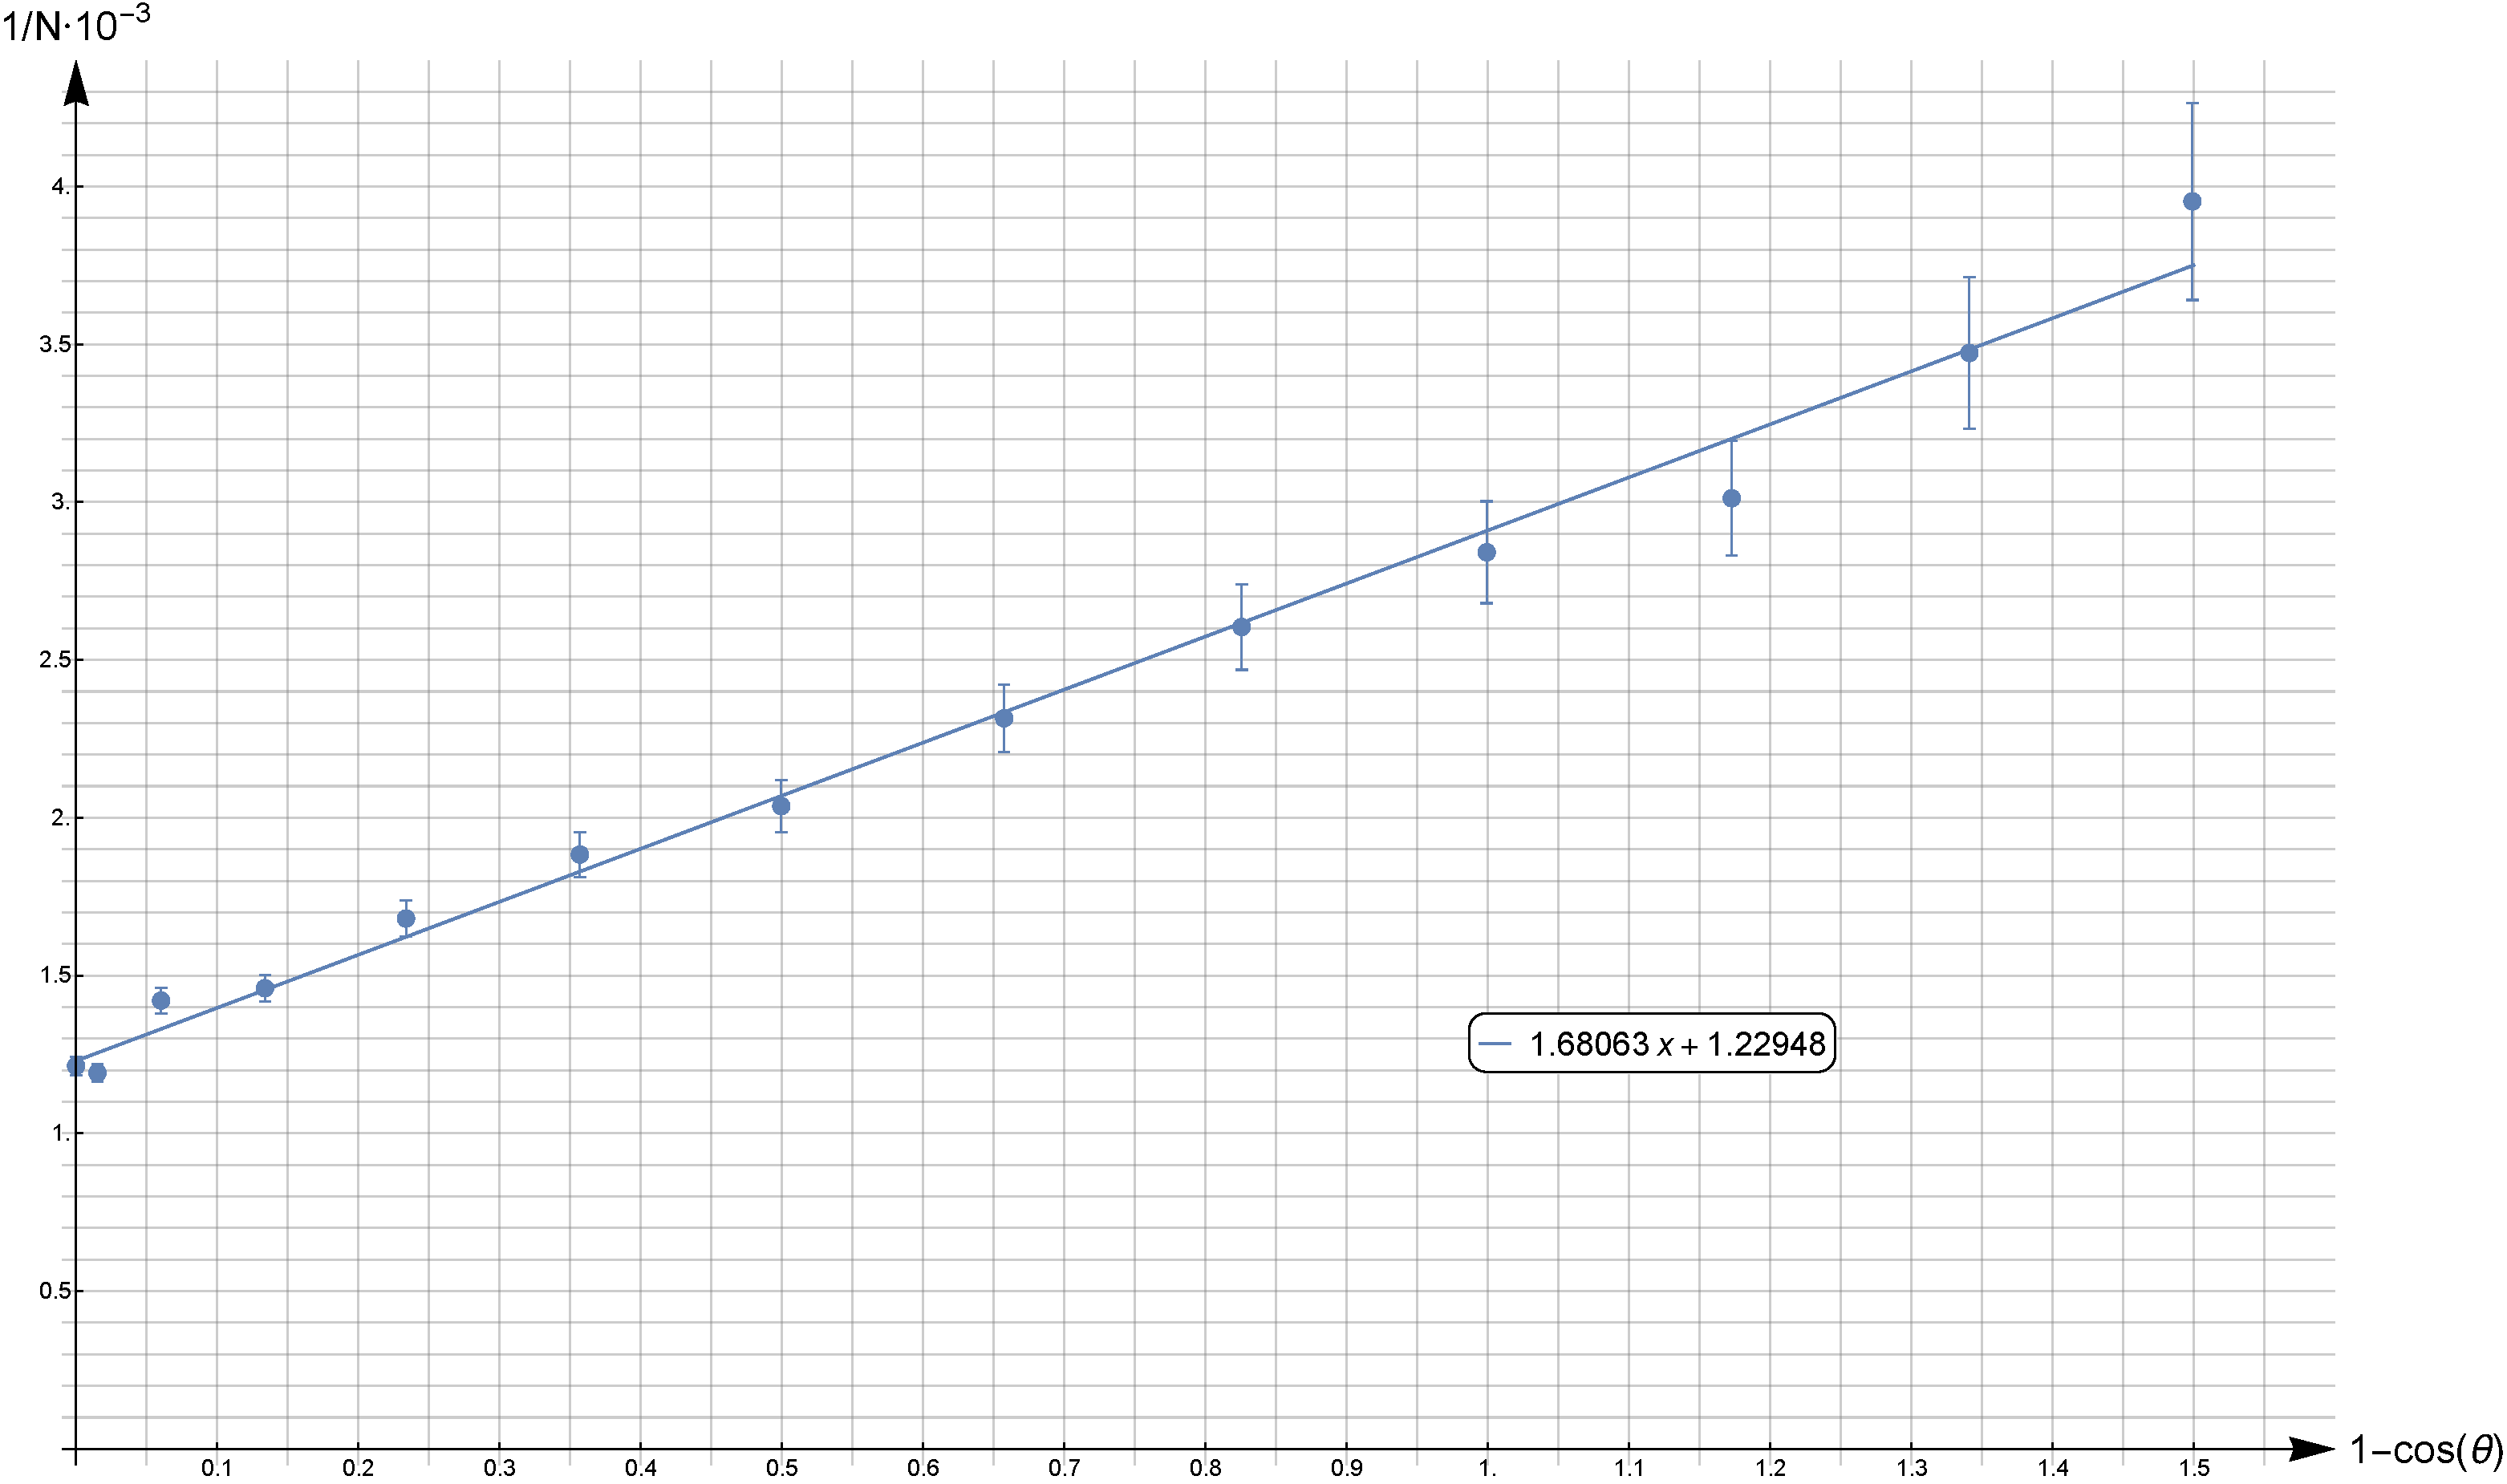
\includegraphics[width=0.9\linewidth]{6}
    \captionsetup{justification=centering}
    \caption{Схема установки для
    исследования газового разряда}
\end{figure}

При подключении к ВИП анода-I между ним
и катодом возникает газовый разряд. Ток
разряда измеряется миллиамперметром $A_1$,
а падение напряжения на разрядной трубке
— цифровым вольтметром $V_1$ (мультиметром
GDM), подключённым к трубке через
высокоомный (25 МОм) делитель напряжения
с коэффициентом $(R_1+R_2)/R_2 = 10$.

При подключении к ВИП анода-II разряд
возникает в пространстве между катодом и
анодом-II, где находится двойной зонд,
используемый для диагностики плазмы
положительного столба. Зонды изготовлены
из молибденовой проволоки диаметром $d =
0,2 \ \text{мм}$ и имеют длину $l = 5,2
\ \text{мм}$. Они
подключены к источнику питания GPS через
потенциометр $R$. Переключатель П$_2$
позволяет изменять полярность напряжения
на зондах. Величина напряжения на зондах
изменяется с помощью дискретного
переключателя <<$V$>> выходного напряжения
источника питания и потенциометра $R$, а
измеряется цифровым вольтметром $V_2$ 
(GDM). Для измерения зондового тока
используется мультиметр $A_2$ (GDM).
Анод-III в нашей работе не используется.

\section{Результаты измерений и обработка результатов}

Установим переключатель П$_1$ в
положение  <<Анод-I>>. Плавно увеличивая
выходное напряжение ВИП, определим
напряжение зажигания разряда (показания
вольтметра перед зажиганием)

\[
    V_\text{з} = (216\pm 3) \ \text{В}
\]

С помощью вольтметра $V_1$ и
амперметра $A_1$ снимем вольт-амперную
характеристику разряда $U_1 = f(I_p)$

\renewcommand{\arraystretch}{1.1} 
\begin{table}[H]
\centering
\begin{tabular}{|c|c|c|c|c|c|c|c|c|c|c|}
\hline
$I_1, \ \text{мА}$ & 0,5   & 0,8   & 1,1   & 1,3   & 1,5   & 1,7   & 1,9   & 2,0   & 2,2   & 2,4   \\ \hline
$U_1, \ \text{В}$ & 34,49 & 33,33 & 32,44
& 31,87 & 30,18 & 27,65 & 25,38 & 24,75
& 23,50 & 22,34 \\ \hline \hline
$I_1, \ \text{мА}$ & 2,6   & 2,9   & 3,2   & 3,5   & 3,7   & 4,0   & 4,2   & 4,4   & 4,7   & 5,0   \\ \hline
$U_1, \ \text{В}$ & 21,69 & 20,93 & 20,45 & 20,00 & 19,81 & 19,61 & 19,52 & 19,44 & 19,31 & 19,18 \\ \hline
\end{tabular}
\captionsetup{justification=centering}
\caption{Вольт-амперная характеристика
разряда}
\end{table}

Построим ВАХ разряда
\begin{figure}[H]
    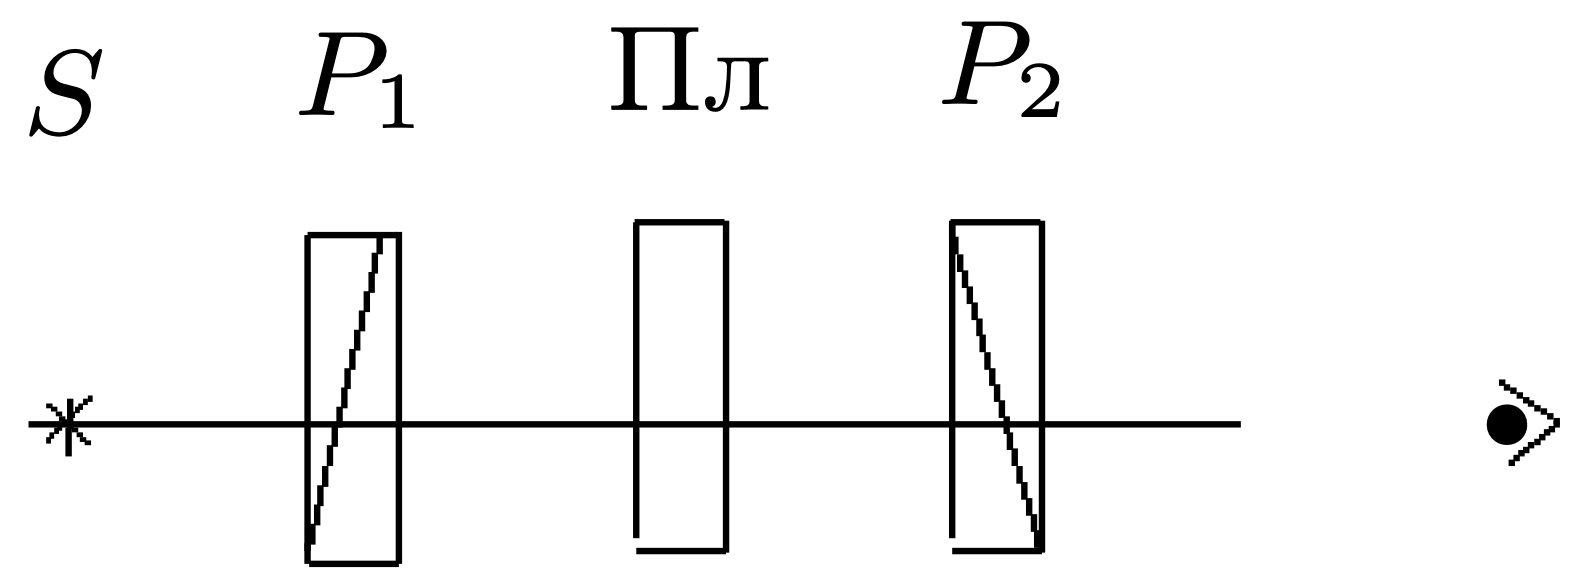
\includegraphics[width=0.9\linewidth]{7}
    \captionsetup{justification=centering}
    \caption{Вольт-амперная
    характеристика разряда $U_1 = f(I_p)$}
\end{figure}

По наклону кривой определим максимальное
дифференциальное сопротивление разряда
$R_{max}$.
\[
    R_{max} = -(10,6 \pm 0,5) \ \text{кОм}
\]

Снимем вольт-амперную характеристику
двойного зонда $I_2 = f(U_2)$ при
фиксированном токе $I_p$

\renewcommand{\arraystretch}{1.2} 

\begin{table}[H]
\centering
\begin{tabular}{|c|c||c|c||c|c|}
\hline
\multicolumn{2}{|c||}{$I_p = 5 \
\text{мА}$} & \multicolumn{2}{c||}{$I_p
= 3 \ \text{мА}$} &
\multicolumn{2}{c|}{$I_p = 1,5 \
\text{мА}$} \\ \hline
$I_2, \ \text{мкА}$  & $U_2, \ \text{В}$
& $I_2, \ \text{мкА}$  & $U_2, \
\text{В}$         & $I_2, \ \text{мкА}$  & $U_2, \ \text{В}$        \\ \hline
109,52      & 25,06     & 60,94      & 25,08     & 31,28      & 25,09     \\ \hline
106,47      & 22,03     & 58,78      & 22,05     & 29,97      & 22,09     \\ \hline
103,42      & 19,07     & 56,62      & 19,01     & 28,69      & 19,07     \\ \hline
99,86       & 16,01     & 54,46      & 16,01     & 27,40      & 16,10     \\ \hline
94,58       & 13,04     & 51,89      & 13,02     & 25,97      & 13,00     \\ \hline
86,20       & 10,05     & 47,93      & 10,02     & 24,02      & 10,02     \\ \hline
78,04       & 8,03      & 43,67      & 8,05      & 21,89      & 8,03      \\ \hline
66,98       & 6,03      & 37,21      & 6,02      & 18,66      & 6,01      \\ \hline
52,46       & 4,01      & 28,35      & 4,02      & 14,29      & 4,08      \\ \hline
35,01       & 2,00      & 16,84      & 2,00      & 8,15       & 2,02      \\ \hline
21,34       & 0,60      & 6,94       & 0,52      & 2,89       & 0,50      \\ \hline
-112,89     & -25,07    & -61,37     & -25,08    & -30,51     & -25,09    \\ \hline
-109,71     & -22,06    & -59,59     & -22,03    & -29,72     & -22,08    \\ \hline
-106,63     & -19,09    & -57,90     & -19,02    & -28,95     & -19,05    \\ \hline
-102,97     & -16,05    & -56,18     & -16,06    & -28,18     & -16,07    \\ \hline
-97,32      & -13,03    & -53,89     & -13,06    & -27,24     & -13,03    \\ \hline
-88,25      & -10,09    & -49,61     & -10,06    & -25,28     & -10,02    \\ \hline
-78,31      & -8,01     & -44,31     & -8,01     & -22,82     & -8,09     \\ \hline
-65,15      & -6,01     & -36,86     & -6,05     & -18,87     & -6,04     \\ \hline
-49,12      & -4,09     & -26,54     & -4,02     & -13,46     & -4,00     \\ \hline
-29,73      & -2,06     & -13,97     & -2,02     & -6,96      & -2,03     \\ \hline
-13,72      & -0,53     & -3,46      & -0,51     & -1,25      & -0,47     \\ \hline
\end{tabular}
\captionsetup{justification=centering}
\caption{Вольт-амперная характеристика
двойного зонда $I_2 = f(U_2)$ при
фиксированном $I_p$}
\end{table}

Определим по графику ток насыщения
$I_{i\text{н}}$ и температуру электронов
при определенном токе разряда $I_p$. По
формуле Бома (20) вычислим концентрацию
электронов $n_e$, полагая, что она равна
концентрации ионов $n_i$. 
\begin{figure}[H]
    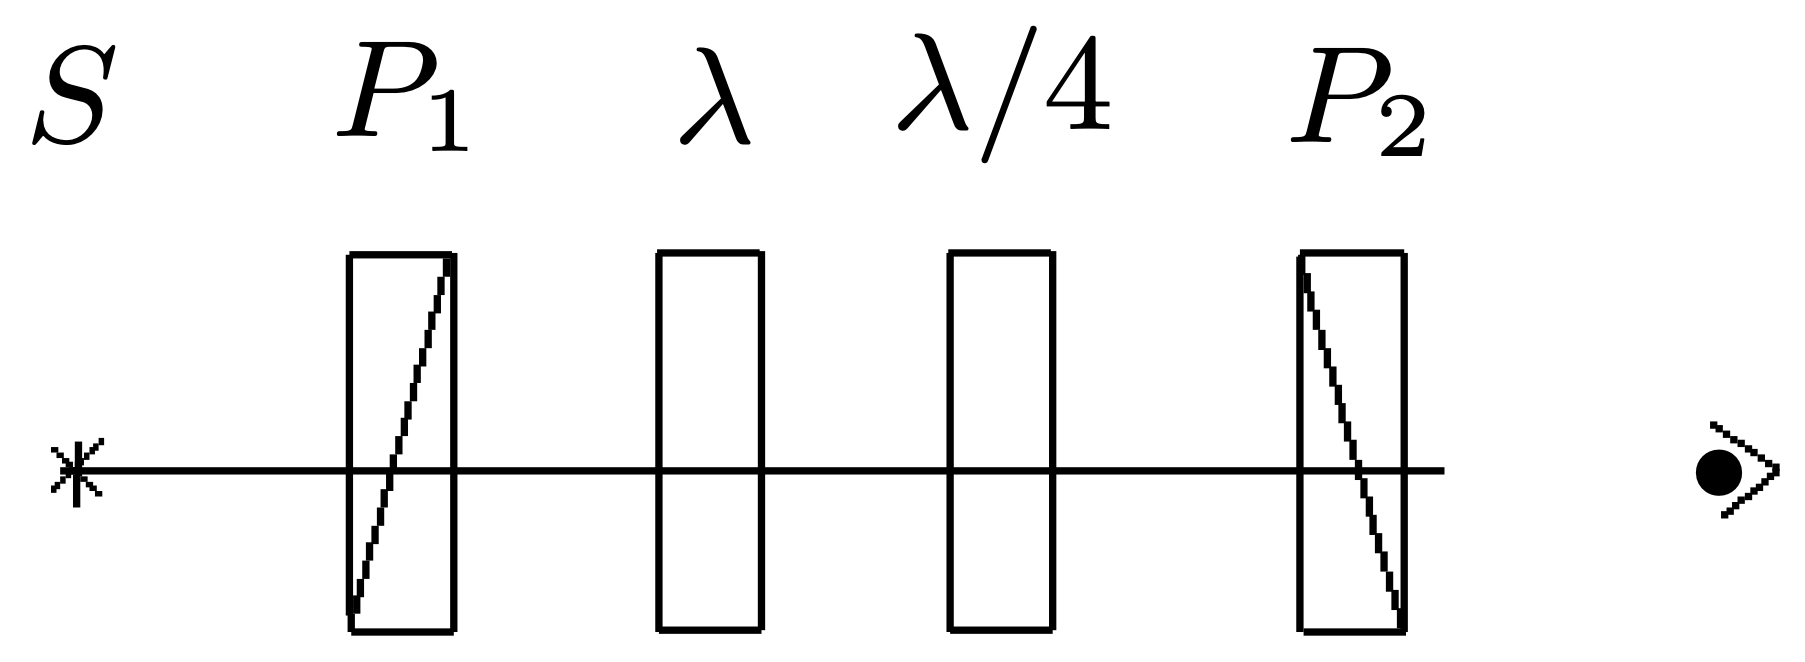
\includegraphics[width=\linewidth]{8}
    \captionsetup{justification=centering}
    \caption{Вольт-амперная характеристика
двойного зонда $I_2 = f(U_2)$ при
фиксированном $I_p$}
\end{figure}

\begin{table}[H]
    \begin{tabular}{|c|c|c|c|}
        \hline
        $I_p, \ \text{мА}$ &
        $I_{i\text{н}}, \ \text{мкА}$ &
        $kT_e, \ \text{эВ}$ & $n_e,
        \ 10^{16} \text{м}^{-3}$ \\ \hline
        5 & $79,7 \pm 1,7$ & $2,3 \pm
        0,4$ &
        $8,39 \pm 0,9$ \\ \hline
        3 & $40,5 \pm 0,9$ & $2,76 \pm
        0,14$
          & $3,92 \pm 0,15$ \\ \hline
        1,5 & $19,6 \pm 0,3$ & $2,91 \pm
        0,08$ & $1,85 \pm 0,06$ \\ \hline
    \end{tabular}
    \captionsetup{justification=centering}
    \caption{Ток насыщения
    $I_{i\text{н}}$, энергия
(температура) электронов $kT_e$ и их
концентрация $n_e$ при заданном токе
разряда $I_p$}
\end{table}

Построим графики $T_e = f(I_p)$,  $n_e =
f(I_p) $

\begin{figure}[H]
    \floatsetup{heightadjust=object,valign=c}
    \begin{floatrow}
        \ffigbox{\captionsetup{justification=centering}\caption{
        График зависимости энергии электронов
$I_e$ от тока разряда $I_p$}}%
        {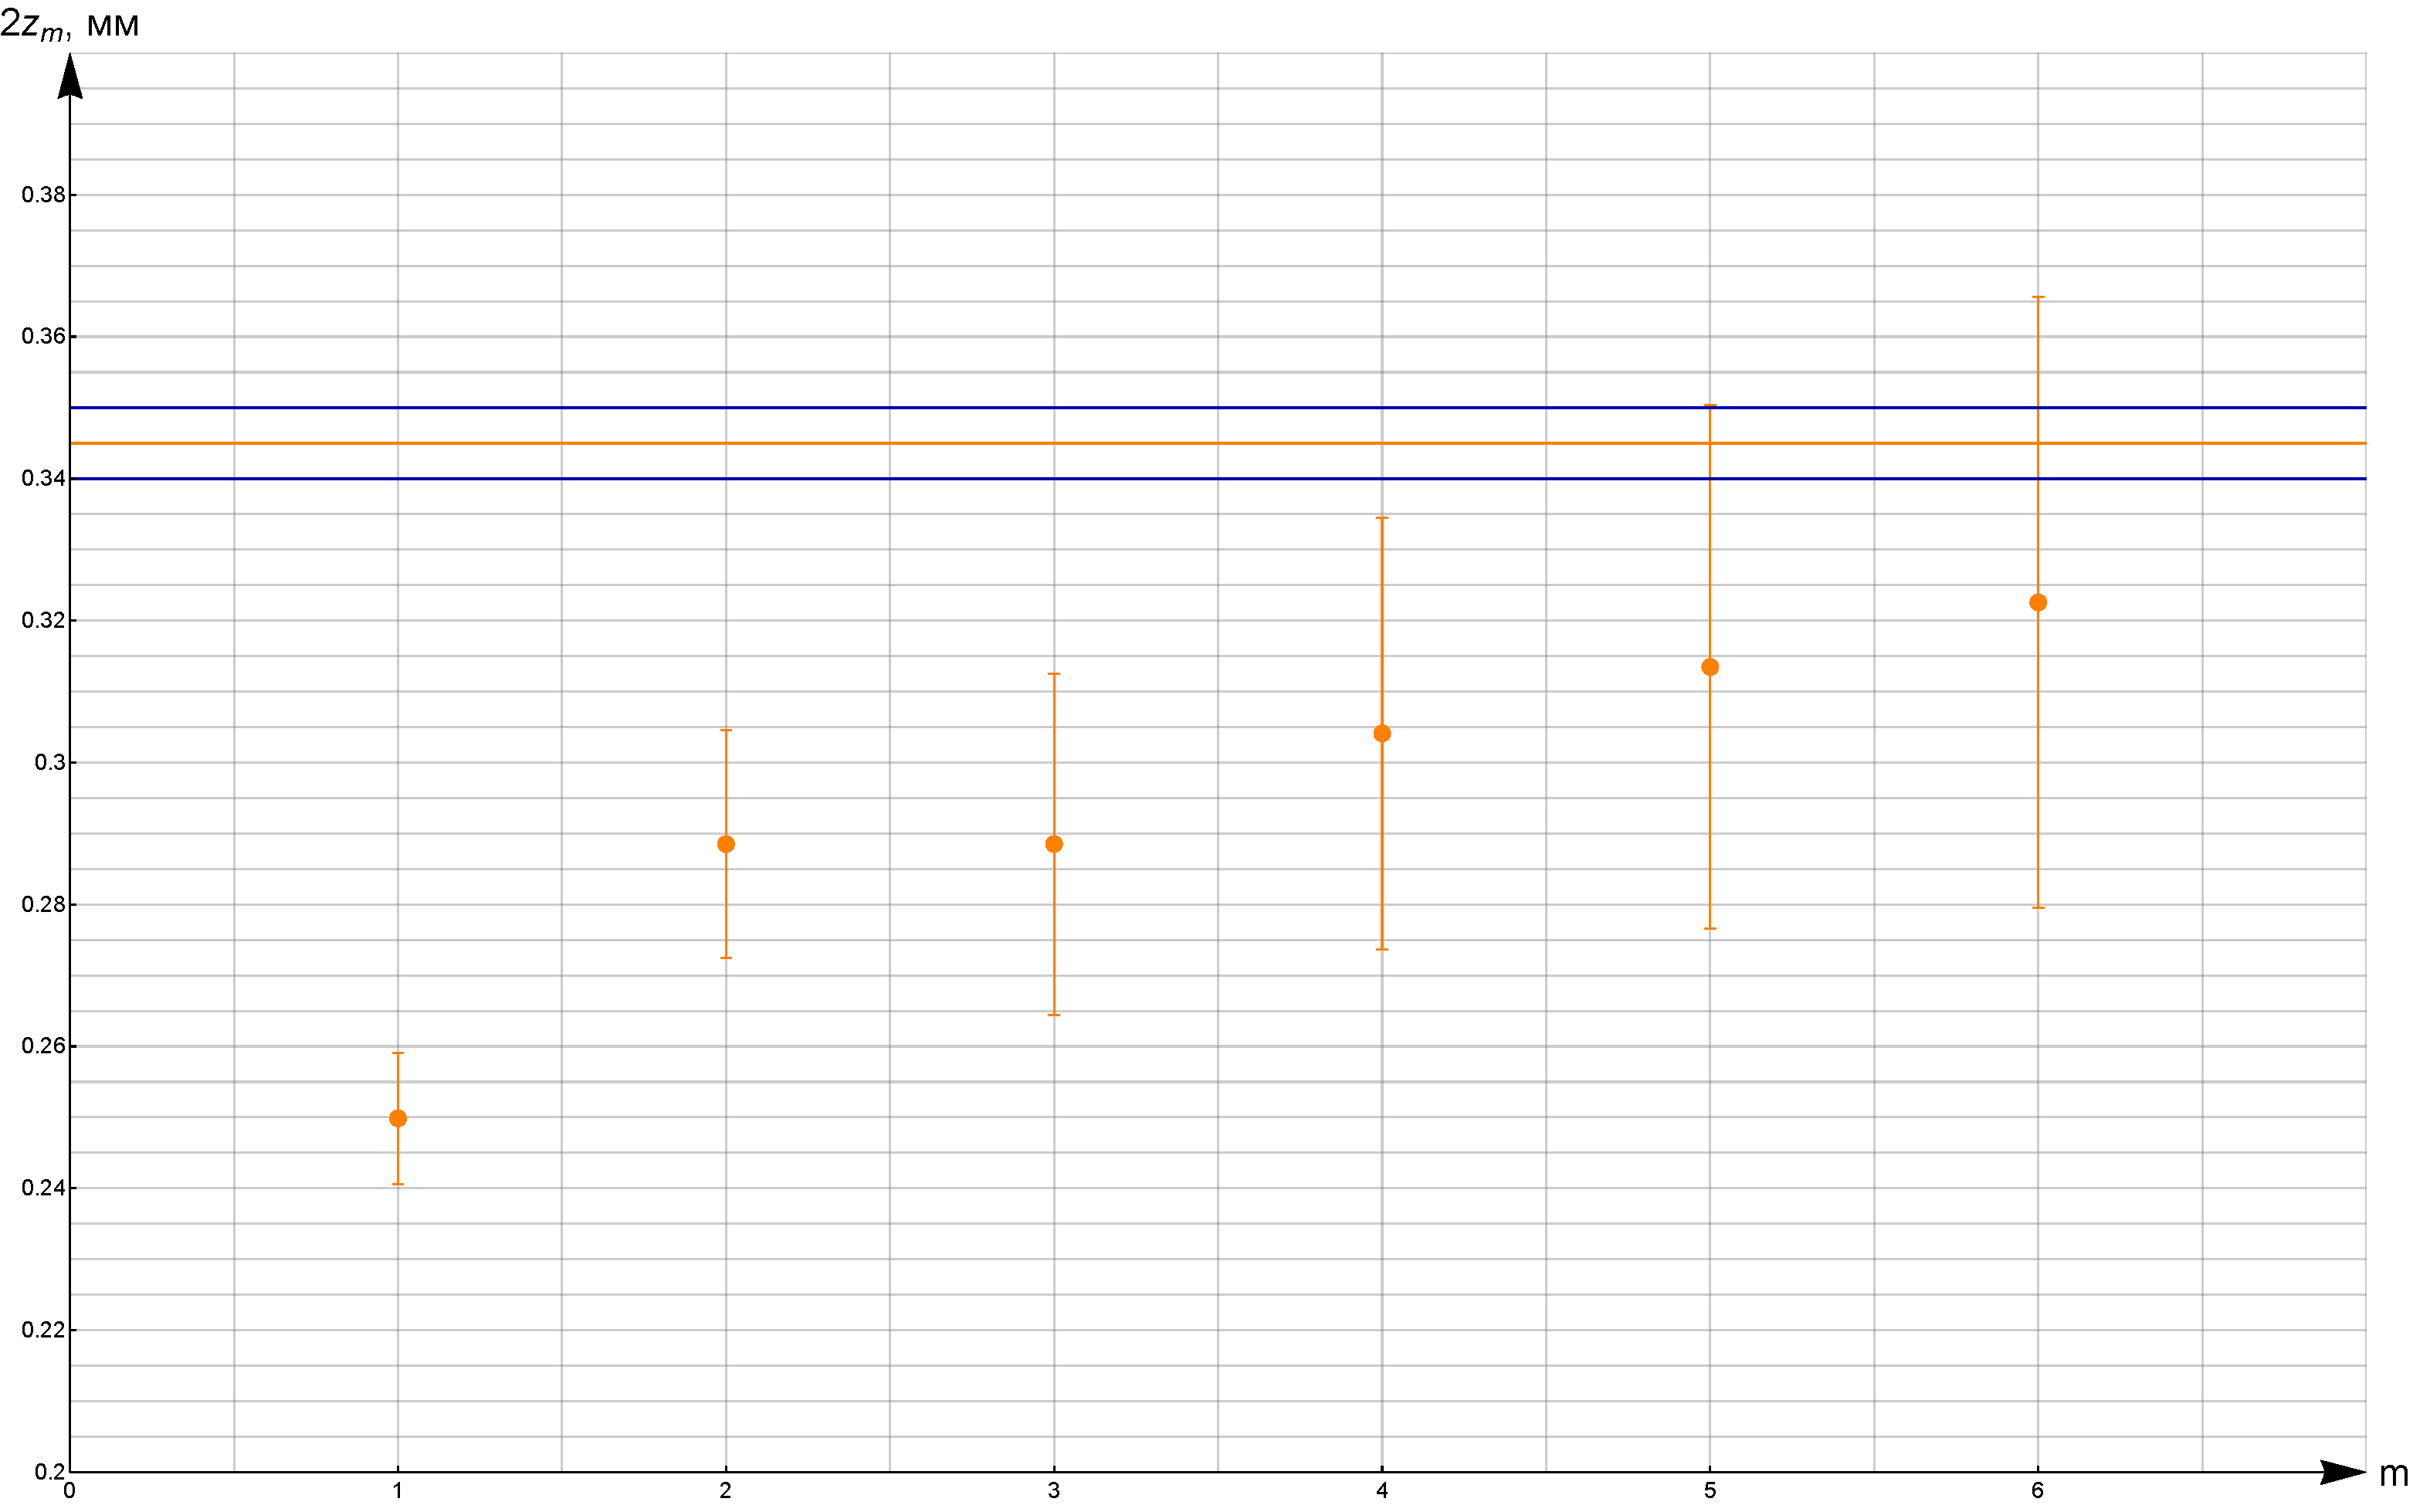
\includegraphics[width
        =\linewidth]{9}}
        \ffigbox{\captionsetup{justification=centering}\caption{График
        зависимости концентрации
электронов $n_e$ от тока разряда $I_p$ }}%
        {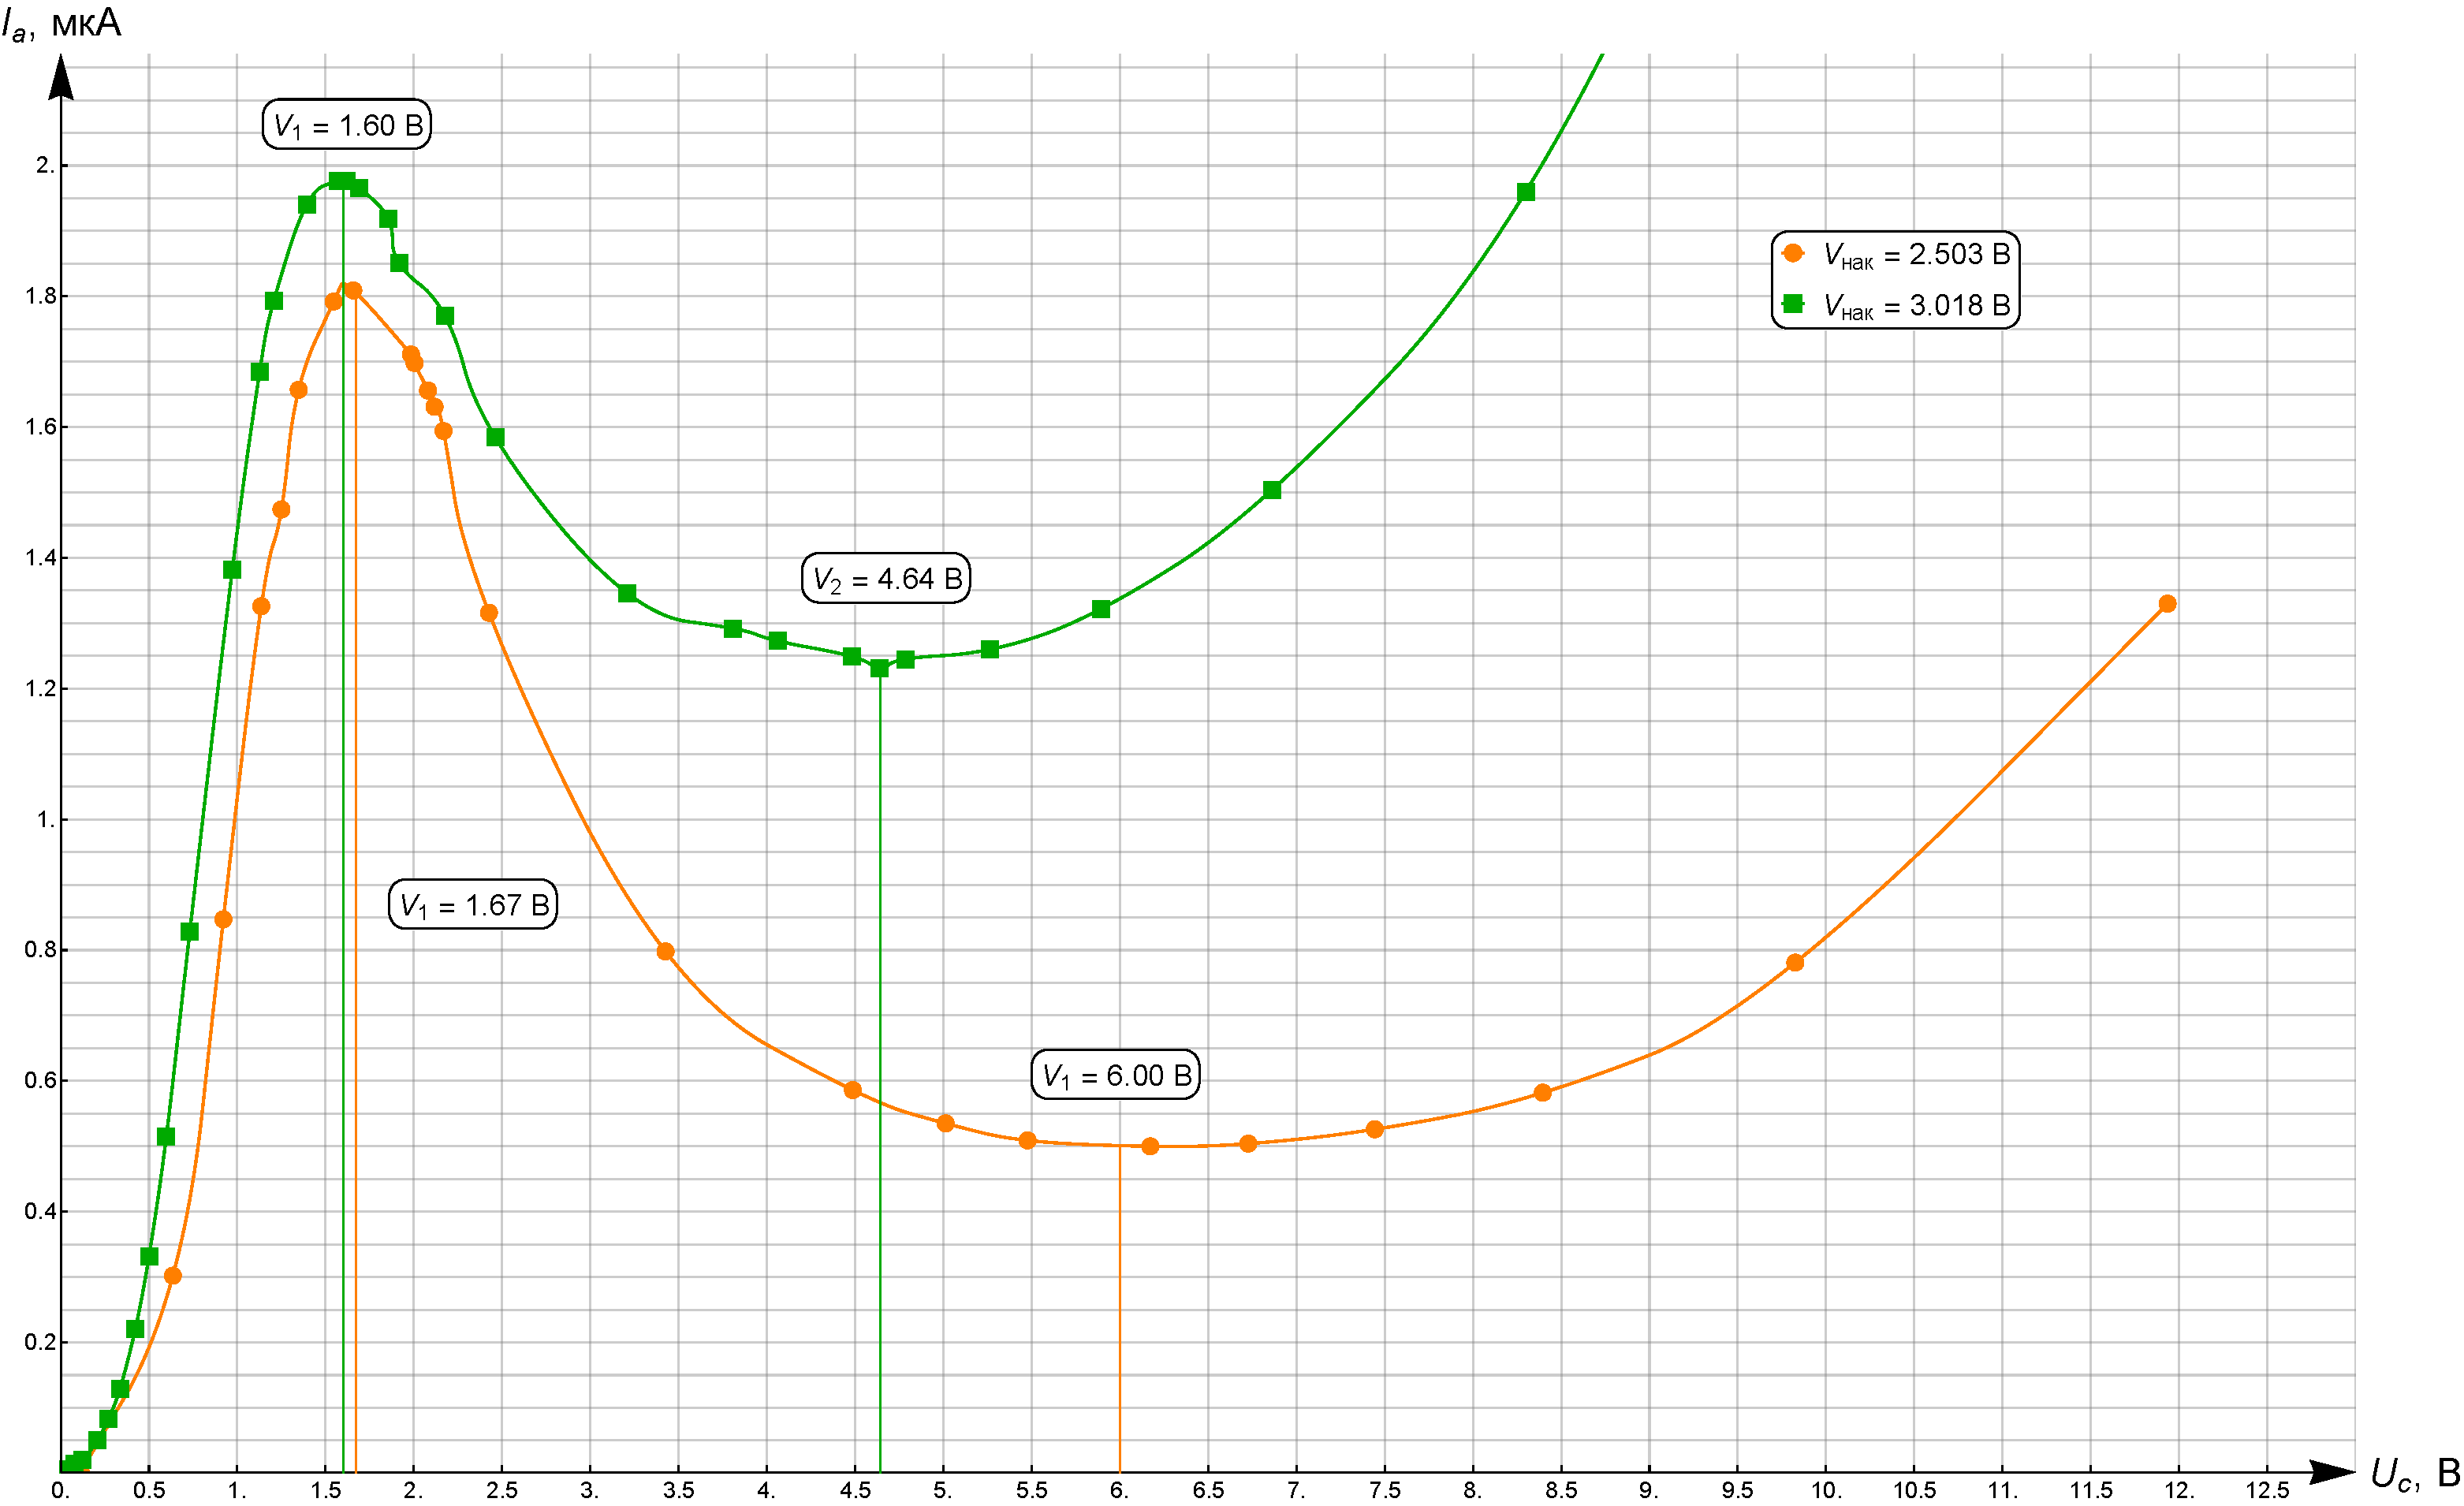
\includegraphics[width=\linewidth]{10}}        
    \end{floatrow}
\end{figure}

Рассчитаем
плазменную частоту колебаний электронов
по формуле (12), также вычислим
дебаевский радиус $r_D$, используя
формулу (14) и условие $T_e \ll T_i$,
$T_i \approx 300 \ \text{К}$. Убедимся,
что среднее число ионов в дебаевской
сфере $N_D \gg 1$ по формуле (8). Оценим
степень ионизации плазмы, если давление
в трубке $P \approx 1 \ \text{мбар}$, а
температура равна комнатной
\[
\alpha = \frac{n_i}{n}
\]
где $n$ -- общее число частиц в единице
объема ($P=nkT$). При нормальных
условиях $n = N_\text{л}$ -- число
Лошмидта.

\begin{table}[H]
    \begin{tabular}{|c|c|c|c|c|}
        \hline
        $I_p, \ \text{мА}$ &
        $\omega_p, \ 10^{10}
        \text{рад/с}$ &
        $r_D, \ 10^{-3}\text{см}$ &
        $N_D, 10^3$ & $\alpha, 10^{-4}$\\ \hline
        5 & $ 1,62 \pm 0,13$ & $3,9 \pm
        0,6$ &
        $21 \pm 6$ & $3,2\pm 0,6$ \\ \hline
        3 & $1,11 \pm 0,03$ & $6,2 \pm
        0,3$
          & $40 \pm 3$ & $1,74 \pm 0,11$\\ \hline
        1,5 & $0,76 \pm 0,02$ & $9,3 \pm
        0,3$ & $62 \pm 4$ & $0,86 \pm
        0,04$ \\ \hline
    \end{tabular}
    \captionsetup{justification=centering}
    \caption{Ленгмюровская частота
    $\omega_p$, дебаевский радиус
$r_D$, среднее число ионов в дебаевской
сфере $N_D$, степень ионизации $\alpha$
при заданном токе разряда  $I_p$}
\end{table}

\section{Обсуждение результатов и выводы}
Результаты расчетов сведем в таблицу:

\renewcommand{\arraystretch}{1.2} 

\begin{table}[H]
    \begin{tabular}{|c|c|c|c|c|}
        \hline
        $I_p, \ \text{мА}$ &
        $I_{i\text{н}}, \ \text{мкА}$ &
        $kT_e, \ \text{эВ}$ & $n_e,
        \ 10^{16} \text{м}^{-3}$ &
        $\omega_p, \ 10^{10}\text{рад/с}$ \\ \hline
        $5,0 \pm 0,1$ & $79,7 \pm 1,7$ & $2,3 \pm
        0,4$ &
        $8,39 \pm 0,9$ & $1,62 \pm 0,13$ \\ \hline
        $3,0 \pm 0,1$ & $40,5 \pm 0,9$ & $2,76 \pm
        0,14$
                      & $3,92 \pm 0,15$
                      & $1,11 \pm 0,03$ \\ \hline
        $1,5 \pm 0,1$ & $19,6 \pm 0,3$ & $2,91 \pm
        0,08$ & $1,85 \pm 0,06$ & $0,76
        \pm 0,02$\\ \hline \hline
        
        $I_p, \ \text{мА}$ &
        $r_D, \ 10^{-3}\text{см}$ &
        $N_D, 10^3$ & $\alpha,
        10^{-4}$\\ \cline{1-4}
        $5,0 \pm 0,1$  & $3,9 \pm
        0,6$ &
        $21 \pm 6$ & $3,2\pm 0,6$ \\
        \cline{1-4}
        $3,0 \pm 0,1$  & $6,2 \pm
        0,3$
          & $40 \pm 3$ & $1,74 \pm
          0,11$\\ \cline{1-4}
        $1,5 \pm 0,1$  & $9,3 \pm
        0,3$ & $62 \pm 4$ & $0,86 \pm
        0,04$ \\ \cline{1-4}
    \end{tabular}
    \captionsetup{justification=centering}
    \caption{Ток насыщения
    $I_{i\text{н}}$, энергия
(температура) электронов $kT_e$, 
концентрация $n_e$, ленгмюровская частота
    $\omega_p$, дебаевский радиус
$r_D$, среднее число ионов в дебаевской
сфере $N_D$, степень ионизации $\alpha$
при заданном токе разряда  $I_p$
}
\end{table}

\end{document}
